\documentclass[10pt,twocolumn,letterpaper]{article}

% ---------------------------------------------------------------- packages
\usepackage[T1]{fontenc}
\usepackage[utf8]{inputenc}
\usepackage{amsmath,amsthm}
\usepackage{newtxtext,newtxmath}
\usepackage[letterpaper,margin=0.75in,columnsep=0.3in]{geometry}
\usepackage{graphicx}
\usepackage{booktabs}
\usepackage{array}
\usepackage{multirow}
\usepackage{xcolor}
\usepackage{listings}
\usepackage{tikz}
\usetikzlibrary{arrows.meta,positioning,fit,calc,backgrounds,decorations.pathreplacing}
\usepackage{algorithm}
\usepackage{algpseudocode}
\usepackage{caption}
\usepackage{subcaption}
\usepackage{enumitem}
\usepackage[numbers,sort&compress]{natbib}
\usepackage[hidelinks]{hyperref}
\usepackage{cleveref}

\captionsetup{font=small,labelfont=bf}
\captionsetup[lstlisting]{justification=raggedright,singlelinecheck=false}
\setlist{nosep,leftmargin=1.2em}
\renewcommand{\labelitemi}{$\bullet$}
\setlength{\abovedisplayskip}{4pt}
\setlength{\belowdisplayskip}{4pt}

\definecolor{r2blue}{HTML}{2a78d6}
\definecolor{r2orange}{HTML}{eb6834}
\definecolor{r2aqua}{HTML}{1baf7a}
\definecolor{r2gray}{HTML}{6f6e69}
\definecolor{r2light}{HTML}{eef4fc}
\definecolor{codebg}{HTML}{f7f7f5}

\lstdefinestyle{py}{
  language=Python, basicstyle=\ttfamily\scriptsize, keywordstyle=\color{r2blue}\bfseries,
  commentstyle=\color{r2gray}\itshape, stringstyle=\color{r2orange!80!black},
  backgroundcolor=\color{codebg}, frame=single, rulecolor=\color{black!12},
  numbers=left, numberstyle=\tiny\color{r2gray}, numbersep=4pt, xleftmargin=10pt,
  breaklines=true, columns=fullflexible, keepspaces=true, showstringspaces=false,
  aboveskip=4pt, belowskip=2pt}
\lstset{style=py}

\newtheorem{proposition}{Proposition}
\newtheorem{corollary}{Corollary}
\theoremstyle{definition}
\newtheorem{definition}{Definition}

\newcommand{\R}{\mathbb{R}}
\newcommand{\Hkv}{H_{\mathrm{kv}}}
\newcommand{\TTFT}{\mathrm{TTFT}}

\hypersetup{pdftitle={R2: A Narrow On-Device Voice Assistant with Persistent Prefix KV Caching},
  pdfauthor={Siavash Shokrtalab, Alireza Panahdoost}}

% ---------------------------------------------------------------- title
\title{\vspace{-1.2em}\Large\bfseries R2: A Narrow, On-Device Voice Assistant with Persistent\\
Prefix KV Caching and Constrained Intent Decoding}

\author{
  \begin{tabular}{c@{\hspace{3em}}c}
  \textbf{Siavash Shokrtalab} & \textbf{Alireza Panahdoost} \\
  Full-stack engineering & Research and machine learning
  \end{tabular}\\[0.5em]
  Department of Computer Engineering, Islamic Azad University, North Tehran Branch, Tehran, Iran\\[0.2em]
  \small Whitepaper, November 2026 (revision 2) \quad$\cdot$\quad Code: \texttt{narrow-ai-with-kv} (MIT License)
}
\date{}

\raggedbottom
\begin{document}
\maketitle

% ---------------------------------------------------------------- abstract
\begin{abstract}
General-purpose assistants pay for their generality with large models, cloud round-trips and loose
control over what they execute. We study the opposite design point: a \emph{narrow} assistant that
maps spoken or typed developer requests to one of eleven validated actions and runs entirely on a
laptop. R2 combines a 4-bit Qwen3-1.7B model on Apple MLX, a \emph{persistent prefix key--value
(KV) cache} for its fixed 1{,}118-token instruction prompt, decoding constrained to the JSON schema
of a decision, and a fail-closed execution layer in which model output is never
authorization. We derive the exactness of prefix reuse for causal decoders, closed-form KV memory
and a roofline-style cost model, and verify them on an Apple M4. Prefix caching reduces end-to-end
time to first token (TTFT) from 1{,}459\,ms to 72\,ms (20.4$\times$) with greedy outputs identical
in 20/20 requests; loading the cache from disk costs 82\,ms instead of a 1.5\,s rebuild. A
context-length sweep shows the forward-pass speed-up growing from 4.5$\times$ at 128 tokens to
85$\times$ at 4{,}096 tokens, matching a fitted cost model ($R^2=0.996$). With strict validation,
R2 is exactly right (intent and parameters) on 92.5\%, 91.7\% and 85.0\% of three evaluation sets
(40 dev, 24 fresh, 60 test requests written last), with 0\% malformed output. An ablation shows
that few-shot examples drive accuracy, constraining only the intent name changes nothing, and a
schema grammar adds 4--12 points by removing every stray parameter. 8-bit KV halves cache memory
at equal accuracy but gives no speed-up; 4-bit KV and short rotating windows break routing.
A LoRA adapter (0.15\% of parameters) trained for 78 minutes on 700 decontaminated synthetic
examples raises exact accuracy on all 124 requests from 88.7\% to 96.8\% (paired McNemar
$p=0.013$) and makes the grammar unnecessary. With Whisper and Kokoro on device, the full voice loop answers in well
under a second. We release the system, a SwiftUI client, benchmarks and notebooks.
\end{abstract}

\noindent\textbf{Index Terms}---KV cache, prefix caching, on-device LLM inference, constrained
decoding, tool use, voice assistants, Apple Silicon, MLX.

% ================================================================ 1 Introduction
\section{Introduction}

Voice assistants such as Siri answer in a fraction of a second because they solve a narrow problem
with specialised models. Large language models (LLMs) promise a more flexible assistant but bring
two costs that matter on a laptop: \emph{latency}, because every request re-reads a long
instruction prompt before producing a single token, and \emph{control}, because a model that can
emit any text can also emit an unintended command.

This whitepaper presents R2, a local, Siri-style assistant for software developers. R2 answers
questions such as ``what's my git status?'', ``find the Swift files'' or ``open Cursor'' by
classifying each request into one of eleven intents with typed parameters, validating it, asking for
confirmation when the action changes something, and speaking a short reply. Its language model is
small (1.7B parameters, 4-bit) and every component---speech recognition, the LLM, speech
synthesis and the tools---runs on the user's Mac.

The key observation is that a narrow assistant's prompt is dominated by a \emph{fixed prefix}: the
instructions, intent catalogue and 25 worked examples occupy 1{,}118 tokens, while a typical request
adds only about 22. Transformer decoders store per-token keys and values (the \emph{KV cache}) that
depend only on earlier tokens, so the prefix can be processed once and reused indefinitely. We make
this cache \emph{persistent}: it is written to disk with a fingerprint so that a restarted
assistant is ready in tens of milliseconds.

\paragraph{Contributions.}
\begin{enumerate}
\item A complete narrow-assistant architecture (\cref{sec:arch}) with a fail-closed authorization
  model in which LLM output only \emph{proposes} actions (\cref{sec:safety}).
\item A formal treatment of prefix KV reuse: an exactness proposition for causal decoders, KV memory
  under grouped-query attention, and a cost model that predicts the speed-up bound
  (\cref{sec:theory}).
\item A persistent prefix cache for MLX whose reuse is keyed on the \emph{content} of the weights,
  tokenizer and adapter and validated layer by layer, and constrained decoders for the intent name
  and for the full decision schema, both failing closed (\cref{sec:impl}).
\item Measurements on an Apple M4: end-to-end cache modes, a context-length sweep, memory, decode,
  disk I/O, accuracy with confidence intervals, an ablation, error analysis and voice latency
  (\cref{sec:results}).
\item A parameter-efficient fine-tuning study: a QLoRA adapter with 0.15\% of the parameters,
  trained on decontaminated synthetic data, compared with the base model under paired tests
  (\cref{sec:lora}).
\item An open implementation with a native macOS client, a terminal interface, reproducible
  benchmark scripts and teaching notebooks (\cref{sec:repro}).
\end{enumerate}

% ================================================================ 2 Background & related work
\section{Background and Related Work}\label{sec:related}

\paragraph{Attention and the KV cache.}
A decoder-only transformer~\cite{vaswani2017attention} computes, in each layer, queries, keys and
values $Q=XW_Q$, $K=XW_K$, $V=XW_V$ and causal attention
$\mathrm{softmax}(QK^\top/\sqrt{d_h}+M)V$, where the mask $M$ forbids attending to future
positions. During autoregressive generation each new token needs the keys and values of all
previous tokens; storing them instead of recomputing them is the KV cache. Pope et
al.~\cite{pope2023efficiently} analyse its memory and latency trade-offs at scale and distinguish the
compute-bound \emph{prefill} phase from the memory-bound \emph{decode} phase, the distinction we use
in \cref{sec:cost}. Multi-query~\cite{shazeer2019fast} and grouped-query attention
(GQA)~\cite{ainslie2023gqa} shrink the cache by sharing key/value heads; Qwen3-1.7B uses GQA with
16 query and 8 KV heads~\cite{yang2025qwen3}. FlashAttention~\cite{dao2022flashattention} makes the
attention computation itself IO-efficient.

\paragraph{Reusing KV state across requests.}
PagedAttention~\cite{kwon2023pagedattention} manages the cache in fixed-size blocks so that
sequences can share memory, which serving systems such as vLLM build on to share common prefixes.
SGLang's RadixAttention~\cite{zheng2024sglang} keeps KV state of past requests in a radix tree with
LRU eviction and reuses the longest matching prefix automatically. Prompt
Cache~\cite{gim2024promptcache} precomputes attention states for reusable \emph{prompt modules} and
reports 8--60$\times$ lower TTFT; because states depend on position, modules must reappear at the
positions they were computed for. CacheBlend~\cite{yao2025cacheblend} relaxes the prefix
requirement for retrieval-augmented generation by selectively recomputing a few tokens of each reused
chunk, and CacheGen~\cite{liu2024cachegen} compresses KV caches into bitstreams so they can be
loaded from storage or the network. llama.cpp~\cite{gerganov2023llamacpp} can save and restore
prompt state to files, and commercial APIs now expose prompt caching with time-limited server-side
caches~\cite{anthropic2024promptcaching}. R2 occupies a simple point in this space: a
\emph{single, fixed} prefix on a \emph{single-user} device, kept in RAM and on disk, with a
content-derived fingerprint and a per-layer shape check that turn any stale or damaged file into a
rebuild rather than a wrong answer.

\paragraph{Shrinking or evicting the cache.}
For long contexts the cache itself becomes the bottleneck. StreamingLLM~\cite{xiao2024streamingllm}
keeps attention-sink tokens plus a sliding window; H$_2$O~\cite{zhang2023h2o} evicts all but
``heavy-hitter'' tokens; KIVI~\cite{liu2024kivi} and KVQuant~\cite{hooper2024kvquant} quantise keys
and values to 2--4 bits. At R2's context lengths (about 1.2k tokens, 140\,MiB) these are not needed,
but they bound how far the design scales (\cref{sec:discussion}).

\paragraph{Structured output.}
Constrained decoding masks tokens that would violate a grammar. Outlines~\cite{willard2023outlines}
compiles regular expressions and JSON schemas into finite-state machines over the vocabulary;
grammar-constrained decoding~\cite{geng2023grammar} applies context-free grammars to structured NLP
tasks; XGrammar~\cite{dong2025xgrammar} makes context-free constraints fast enough for serving; and
LMQL~\cite{beurer2023lmql} treats prompting as constrained programming. R2 first used the lightest
form, a mask over the intent name only; it now compiles the whole decision schema to a grammar with
llguidance~\cite{llguidance2025} and still validates the result afterwards (\cref{sec:constrained}).

\paragraph{Tool use and assistants.}
Toolformer~\cite{schick2023toolformer}, ReAct~\cite{yao2023react} and
Gorilla~\cite{patil2024gorilla} teach LLMs to call tools or APIs. These systems maximise breadth;
R2 deliberately minimises it, so that a 1.7B model reaches high accuracy through few-shot
prompting~\cite{brown2020language} alone, an optional LoRA adapter~\cite{hu2022lora} adds the
rest (\cref{sec:lora}), and every call passes a deterministic policy check.

\paragraph{Parameter-efficient fine-tuning.}
Adapter layers~\cite{houlsby2019adapters} insert small trainable modules between frozen layers;
prefix-tuning~\cite{li2021prefix} learns continuous vectors prepended to every layer's keys and
values; LoRA~\cite{hu2022lora} learns a low-rank update to frozen weight matrices, motivated by
the observation that fine-tuning has a low intrinsic dimension~\cite{aghajanyan2021intrinsic};
QLoRA~\cite{dettmers2023qlora} trains LoRA on top of a 4-bit base model. \Cref{sec:lora} explains
why LoRA is the variant that fits R2.

\paragraph{On-device models.}
Post-training quantisation such as GPTQ~\cite{frantar2023gptq} and AWQ~\cite{lin2024awq} makes
billion-parameter models practical on laptops. MLX~\cite{hannun2023mlx} is an array framework for
Apple Silicon's unified memory, and mlx-lm provides model implementations, quantised weights and
prompt-cache utilities. For speech, R2 uses Whisper~\cite{radford2023whisper} for recognition and
Kokoro-82M~\cite{hexgrad2024kokoro}, a compact model in the StyleTTS~2
family~\cite{li2023styletts2}, for synthesis.

\Cref{tab:related} summarises how R2's cache compares with these systems.

\begin{table*}[t]
\centering\small
\caption{Prefix and KV reuse in related systems. ``Restart'' = the reused state survives a restart
of the serving process. Entries describe each system's published design, not every configuration.}
\label{tab:related}
\footnotesize
\begin{tabular}{@{}>{\raggedright\arraybackslash}p{3.0cm}>{\raggedright\arraybackslash}p{3.1cm}>{\raggedright\arraybackslash}p{2.4cm}c>{\raggedright\arraybackslash}p{4.3cm}>{\raggedright\arraybackslash}p{2.6cm}@{}}
\toprule
System & Reuse unit & Where stored & Restart & Reuse condition / validity check & Target setting \\
\midrule
PagedAttention / vLLM~\cite{kwon2023pagedattention} & fixed-size KV blocks & GPU memory & -- & hash of the block's token prefix & multi-tenant serving \\
SGLang RadixAttention~\cite{zheng2024sglang} & longest cached token prefix & GPU / host memory & -- & radix-tree prefix match, LRU & multi-tenant serving \\
Prompt Cache~\cite{gim2024promptcache} & reusable prompt modules & GPU / CPU memory & -- & module schema fixes positions & serving, research \\
CacheBlend~\cite{yao2025cacheblend} & any text chunk & GPU / CPU / storage & \checkmark & selective recompute of a few tokens & retrieval-augmented generation \\
CacheGen~\cite{liu2024cachegen} & compressed KV bitstream & network / disk & \checkmark & lossy encoding, quality-controlled & context loading over networks \\
llama.cpp~\cite{gerganov2023llamacpp} & whole prompt / session state & file & \checkmark & saved tokens must match the prompt & local, single user \\
Provider APIs~\cite{anthropic2024promptcaching} & marked prompt prefixes & provider servers, TTL & -- & exact prefix match & cloud APIs \\
\textbf{R2 (ours)} & \textbf{fixed system prefix; conversation prefix (opt.)} & \textbf{RAM (LRU 4) + disk (LRU 8)} & \checkmark & \textbf{content hash of weights, tokenizer, template, adapter; per-layer shape check} & \textbf{single-user laptop} \\
\bottomrule
\end{tabular}
\end{table*}

% ================================================================ 3 Why not existing solutions
\section{Aren't Existing Solutions Good Enough?}\label{sec:why}

A developer who wants to ask their laptop ``what's my git status?'' by voice has four kinds of
existing tools. Each meets some of the requirements below, none meets all of them, and the gaps
are measurable on our own hardware.

\begin{table}[t]
\centering\small
\caption{Requirements met by typical configurations of each approach (\checkmark{} yes,
$\circ$ partly or depends on configuration, -- no). Q1 on-device and private; Q2 first token
${<}100$\,ms on a laptop; Q3 typed, validated decisions; Q4 model output never authorises an
action; Q5 developer-workspace actions; Q6 fast again after a restart.}
\label{tab:why}
\setlength{\tabcolsep}{4pt}
\begin{tabular}{@{}lcccccc@{}}
\toprule
Approach & Q1 & Q2 & Q3 & Q4 & Q5 & Q6 \\
\midrule
OS voice assistant & $\circ$ & \checkmark & \checkmark & \checkmark & -- & \checkmark \\
Cloud LLM agent & -- & $\circ$ & $\circ$ & $\circ$ & \checkmark & $\circ$ \\
Local chat runtime & \checkmark & -- & $\circ$ & -- & -- & $\circ$ \\
Serving engine & $\circ$ & \checkmark & $\circ$ & -- & -- & -- \\
\textbf{R2} & \checkmark & \checkmark & \checkmark & \checkmark & \checkmark & \checkmark \\
\bottomrule
\end{tabular}
\end{table}

\paragraph{OS voice assistants} are fast and constrained to typed intents, which is why their
actions are safe. But their intent catalogue is fixed by the vendor and knows nothing about a
developer's repository, files or tools, and part of the processing may happen on servers.

\paragraph{Cloud LLM assistants and coding agents} are capable and know developer workflows, but
every request crosses the network and sends workspace content off the device. Many give the model
broad tools, sometimes a shell, so that text read from a file or web page can steer an action
(indirect prompt injection~\cite{greshake2023injection}); whether that is prevented depends on the
harness, not the model. Their prompt caches live on the provider's servers with a time limit.

\paragraph{Local chat runtimes} (built, for example, on llama.cpp~\cite{gerganov2023llamacpp}) keep
data on the device, but they are general chat front ends: they have no notion of a validated action,
and a narrow assistant built naively on them re-reads its long instruction prompt on every request.
With R2's own model and prompt that costs 1{,}459\,ms before the first token
(\cref{tab:kvmodes}), and free decoding of the 1.7B model produces stray parameters that strict
validation must reject in 6.7--20\% of test requests (\cref{tab:ablation3}).

\paragraph{Serving engines} with prefix caching (vLLM, SGLang; \cref{tab:related}) solve the
latency problem for many users on a server GPU. They keep the cache in memory of a long-running
process and have no execution policy; on a laptop, where the assistant is started and stopped
with the user's session, the cache would be rebuilt after every restart.

\paragraph{What R2 changes.} R2 combines the parts each approach gets right and closes the gaps
with mechanisms we can measure: a persistent, fingerprinted prefix cache (72\,ms to the first
token, 82\,ms to load after a restart; \cref{sec:results}), decoding constrained to the decision
schema plus strict validation (0\% malformed output, 0\% fallbacks), an optional LoRA adapter that
raises exact accuracy to 96.8\% (\cref{sec:lora}), and an executor in which the model only
\emph{proposes} actions while allow-lists, workspace guards and user confirmation decide
(\cref{sec:safety}). The price is breadth: R2 knows eleven intents and declines everything else.

% ================================================================ 4 Problem formulation
\section{Problem Formulation}\label{sec:problem}

Let $\mathcal{I}$ be a finite set of intents, here $|\mathcal{I}|=11$: \texttt{git\_status},
\texttt{git\_diff\_summary}, \texttt{search\_files}, \texttt{read\_file}, \texttt{open\_app},
\texttt{remember\_preference}, \texttt{recall\_preference}, \texttt{answer\_question},
\texttt{general\_help}, \texttt{clarify\_request} and \texttt{unsupported}. Each intent
$i\in\mathcal{I}$ has a parameter schema $\Theta_i$ (for example $\Theta_{\texttt{search\_files}}$
is a glob pattern). Given an utterance $u$ and a short history $h$, the assistant must produce a
\emph{decision} $d=(i,\theta)$ with $\theta\in\Theta_i$, and then either execute it, ask for
confirmation, ask for clarification or decline.

We optimise three objectives in priority order:
\begin{enumerate}
\item \textbf{Safety:} no action executes unless it is valid, allow-listed, inside the workspace
  and, for privileged actions, confirmed by the user (\cref{sec:safety}).
\item \textbf{Accuracy:} the predicted intent and parameters match a reference.
\item \textbf{Latency:} minimise time to first token (TTFT) and total decision latency, since the
  intent name is fully determined within the first few generated tokens.
\end{enumerate}

The language model $p_\phi$ defines $d$ through its output string $y$. R2 restricts $y$ either to
start with the prefill $\pi=$\,\texttt{\{"intent": "} followed by a name in $\mathcal{I}$
(\emph{intent} mode) or, by default, to the language of the decision schema (\emph{json} mode).

% ================================================================ 4 Theory
\section{Theoretical Analysis}\label{sec:theory}

\subsection{Prefix invariance of causal decoders}

Let $x_{1:N}$ be a token sequence, $L$ the number of layers and $h^{(\ell)}_t\in\R^{d}$ the hidden
state of token $t$ after layer $\ell$, with $h^{(0)}_t=E[x_t]$. With rotary position embeddings
(RoPE)~\cite{su2024roformer} applied at absolute position $t$, layer $\ell$ computes for each KV
head $g$
\begin{align}
k^{(\ell,g)}_t &= \mathrm{RoPE}_t\!\left(W_K^{(\ell,g)}\,\mathrm{norm}(h^{(\ell-1)}_t)\right),\label{eq:k}\\
v^{(\ell,g)}_t &= W_V^{(\ell,g)}\,\mathrm{norm}(h^{(\ell-1)}_t),\label{eq:v}
\end{align}
and each query head $j$ (mapped to KV head $g(j)$) attends only to positions $\le t$:
\begin{equation}
o^{(\ell,j)}_t=\sum_{\tau\le t}\frac{\exp\!\big(q^{(\ell,j)\top}_t k^{(\ell,g(j))}_\tau/\sqrt{d_h}\big)}
{\sum_{\tau'\le t}\exp\!\big(q^{(\ell,j)\top}_t k^{(\ell,g(j))}_{\tau'}/\sqrt{d_h}\big)}\,
v^{(\ell,g(j))}_\tau.\label{eq:attn}
\end{equation}

\begin{proposition}[Prefix invariance]\label{prop:prefix}
For every layer $\ell$ and position $t\le p$, the keys $k^{(\ell,\cdot)}_t$ and values
$v^{(\ell,\cdot)}_t$ depend only on the prefix $x_{1:p}$ and not on any later token.
\end{proposition}
\begin{proof}
By induction on $\ell$. For $\ell=1$, $k^{(1)}_t,v^{(1)}_t$ are functions of $h^{(0)}_t=E[x_t]$ and
of $t$ only. Assume that for layer $\ell$ every $h^{(\ell-1)}_\tau$ with $\tau\le t$ depends only on
$x_{1:t}$. Then \cref{eq:k,eq:v} make $k^{(\ell)}_t,v^{(\ell)}_t$ functions of $x_{1:t}$, and
\cref{eq:attn} sums only over $\tau\le t$, so $o^{(\ell)}_t$ and hence $h^{(\ell)}_t$ (after the
residual connection and MLP, which act position-wise) depend only on $x_{1:t}$. Taking $t\le p$
completes the induction.
\end{proof}

\begin{corollary}[Exact reuse]\label{cor:exact}
Let $C(x_{1:p})$ be the per-layer keys and values of a prefix. For any suffix $x_{p+1:p+s}$, running
the model on $x_{p+1:p+s}$ with cache $C(x_{1:p})$ yields, in exact arithmetic, the same logits as
running it on $x_{1:p+s}$ from scratch, provided the suffix is placed at positions $p+1,\dots,p+s$.
\end{corollary}

The positional proviso is why Prompt Cache must keep modules at fixed positions~\cite{gim2024promptcache}
and why CacheBlend needs recomputation for non-prefix chunks~\cite{yao2025cacheblend}. R2 always
places its cached text at the start of the prompt, so the corollary applies directly. In floating
point the two computations use different kernel shapes and summation orders, so logits can differ
in low-order bits; \cref{sec:equiv} measures this.

\begin{corollary}[Longest common prefix]\label{cor:lcp}
Let $x$ be a sequence whose cache $C(x)$ is stored and $x'$ a new sequence, and let
$\ell=\mathrm{LCP}(x,x')$ be the length of their longest common token prefix. Trimming $C(x)$ to its
first $\ell$ positions gives exactly $C(x'_{1:\ell})$, so only $|x'|-\ell$ tokens need prefilling.
\end{corollary}
\begin{proof}
By \cref{prop:prefix}, positions $t\le\ell$ of both caches depend only on $x_{1:\ell}=x'_{1:\ell}$.
\end{proof}

\noindent Conversation-level reuse (\cref{sec:convreuse}) applies \cref{cor:lcp} across turns. Its
gain is set by $\ell$, which depends on how history is cut: dropping the oldest turn changes the
token right after the system prompt, so $\ell$ falls back to the prefix length $p$ and nothing is
saved. A \emph{rotating} window of $W$ positions with $k$ retained ``sink'' tokens violates the
premise of \cref{cor:exact} instead: once $|x|>W$, the last position attends only to
$x_{1:k}\cup x_{|x|-W+k+1:|x|}$, so for $W<p$ the request no longer sees most of the instructions,
whatever the cache holds (\cref{sec:kvvariants}).

\subsection{KV cache memory}\label{sec:memory}

Each cached token stores one key and one value vector per layer and KV head. With $b$ bytes per
element,
\begin{equation}
M(n)=2\,L\,\Hkv\,d_h\,b\,n .\label{eq:mem}
\end{equation}
For Qwen3-1.7B ($L=28$, $\Hkv=8$, $d_h=128$) in bfloat16 ($b=2$) this is
$2\cdot28\cdot8\cdot128\cdot2=114{,}688$\,B $=112$\,KiB per token. Without GQA (16 KV heads) the
cache would be twice as large; the saving factor is $H/\Hkv=2$. mlx-lm grows the cache in steps of
$\kappa=256$ tokens, so the allocated size is
\begin{equation}
M_{\text{alloc}}(n)=2\,L\,\Hkv\,d_h\,b\,\kappa\left\lceil n/\kappa\right\rceil .\label{eq:alloc}
\end{equation}
R2's 1{,}118-token prefix therefore occupies $5\cdot256=1{,}280$ slots, i.e.\ 140\,MiB
(146.8\,MB), which is exactly the size of the cache file R2 writes. For comparison, the 4-bit
weights occupy about 0.94\,GB, so the cache adds 15\%.

\paragraph{Quantised KV.} Affine quantisation to $\beta$ bits in groups of $g$ elements stores, per
group, one scale and one bias in the original precision ($b$ bytes each), so
\begin{equation}
M_\beta(n)=2\,L\,\Hkv\,d_h\left(\frac{\beta}{8}+\frac{2b}{g}\right)n,\qquad
\frac{M_\beta}{M}=\frac{\beta/8+2b/g}{b}. \label{eq:memq}
\end{equation}
With $b=2$ and $g=64$ the ratio is $0.531$ for $\beta=8$ and $0.281$ for $\beta=4$, predicting
78.0 and 41.3\,MB for R2's allocated prefix; both match the measured sizes exactly
(\cref{sec:kvvariants}). By \cref{eq:tdec} the cache term of decoding shrinks by the same ratio,
but at $n\le8\text{k}$ it is small next to reading the weights, so little speed is to be gained.

\subsection{A cost model for prefill and decode}\label{sec:cost}

Following the roofline view~\cite{williams2009roofline,pope2023efficiently}, prefill of $N$ tokens is
compute-bound and decode is memory-bound. Let $P$ be the number of parameters touched per token
(including the language-model head) and $H$ the number of query heads. A causal prefill costs
\begin{equation}
F_{\text{pre}}(N)\approx\underbrace{2PN}_{\text{matmuls}}+\underbrace{2LHd_hN^2}_{\text{attention}}
\label{eq:flops}
\end{equation}
FLOPs, where the attention term counts $QK^\top$ and $AV$ ($2\times2LHd_h$ per query--key pair)
over the $N^2/2$ causal pairs. With effective throughput $\Pi$ and a fixed overhead $a$ (kernel
launches, synchronisation), the prefill time is
\begin{equation}
T_{\text{pre}}(N)=a+bN+cN^2,\quad b=\frac{2P}{\Pi},\quad c=\frac{2LHd_h}{\Pi}. \label{eq:tpre}
\end{equation}
A \emph{cached} prefill of $s$ new tokens after a prefix of length $n$ touches the weights $s$
times and attends from $s$ queries to $n+s$ keys:
\begin{equation}
T_{\text{suf}}(s\mid n)=\alpha+bs+4LHd_h\frac{s\,n+s(s+1)/2}{\Pi}\;\approx\;\alpha+\gamma n
\label{eq:tsuf}
\end{equation}
for fixed $s$. Decoding one token with $n$ cached tokens reads all weights $W$ bytes and the cache,
\begin{equation}
T_{\text{dec}}(n)=d_0+d_1 n,\quad d_0\approx\frac{W}{B},\quad d_1\approx\frac{2L\Hkv d_h b}{B},
\label{eq:tdec}
\end{equation}
where $B$ is the achieved memory bandwidth.

\subsection{Speed-up of prefix caching}\label{sec:speedup}

The TTFT speed-up of caching a length-$n$ prefix for an $s$-token suffix is
\begin{equation}
S(n,s)=\frac{T_{\text{pre}}(n+s)}{T_{\text{suf}}(s\mid n)}
=\frac{a+b(n+s)+c(n+s)^2}{\alpha+bs+O(sn)/\Pi}. \label{eq:speedup}
\end{equation}
If overheads vanish ($a=\alpha=0$) and attention is negligible ($c\to0$), the speed-up is the
token ratio
\begin{equation}
S^\star(n,s)=\frac{n+s}{s}, \label{eq:bound}
\end{equation}
which for R2 ($n=1{,}118$, $s=22$) is 51.8. Two effects push the measured value below
$S^\star$: the fixed cost $\alpha$ of a forward pass, which dominates when $s$ is small, and
per-request work outside the model (tokenisation, sampling, constraint masks). Conversely, for long
prefixes the quadratic term makes $S$ grow faster than linearly. The crossover length at which
attention costs as much as the matrix multiplications is $N^\star=b/c=P/(LHd_h)$.

\paragraph{Amortisation.}
Building the prefix costs one uncached prefill, $T_{\text{pre}}(n)$; each later request saves
$\Delta=T_{\text{pre}}(n+s)-T_{\text{suf}}(s\mid n)$. In memory, caching pays for itself after
$\lceil T_{\text{pre}}(n)/\Delta\rceil=2$ requests. On disk, the build cost is replaced by a load
cost $T_{\text{load}}\approx M_{\text{alloc}}(n)/B_{\text{disk}}$, paid once per process start.

\subsection{Constrained intent decoding}\label{sec:constrained}

Let $\mathcal{V}$ be the vocabulary, $\sigma(v)$ the string of token $v$, and
$\mathcal{W}=\{w\,\Vert\,\texttt{"} : w\in\mathcal{I}\}$ the target strings (each intent name
followed by its closing quote). After the prefill $\pi$, let $y_{<t}$ be the text generated so far.
Write $a\preceq b$ if $a$ is a prefix of $b$.

\begin{definition}[Allowed set]
\begin{equation}
A(y_{<t})=\{v\in\mathcal{V}:\exists w\in\mathcal{W},\;y_{<t}\sigma(v)\preceq w\;\lor\;w\preceq y_{<t}\sigma(v)\}.
\end{equation}
\end{definition}

The decoder replaces the logits $z_v$ by $z'_v=z_v$ for $v\in A(y_{<t})$ and $-\infty$ otherwise,
so the sampling distribution becomes
\begin{equation}
p'(v\mid y_{<t})=\frac{p(v\mid y_{<t})\,\mathbf{1}[v\in A(y_{<t})]}{\sum_{u\in A(y_{<t})}p(u\mid y_{<t})}.
\end{equation}
Masking stops as soon as some $w\in\mathcal{W}$ is a prefix of the generated text.

\begin{proposition}[Soundness]
If $A(y_{<t})\neq\emptyset$ at every masked step, the generated intent name is an element of
$\mathcal{I}$.
\end{proposition}
\begin{proof}
By construction every masked step keeps $y_{\le t}$ consistent with some target $w$, i.e.\ either a
prefix of $w$ or extending it. Since targets end with a quote that cannot occur inside a name, the
first time a full target is a prefix of $y$ the name equals some $w\in\mathcal{I}$, and masking
stops.
\end{proof}

With greedy decoding, the choice becomes $\arg\max_{v\in A}z_v$, so masking can only change the
output when the unconstrained argmax would have left $\mathcal{I}$. The mask is computed once per
distinct prefix and memoised; candidate tokens are pre-filtered to those whose characters all occur
in some target, so each step costs $O(|\mathcal{V}'|)$ with $|\mathcal{V}'|\ll|\mathcal{V}|$.
If $A(y_{<t})=\emptyset$ the precondition fails, so the decoder then allows only end-of-sequence
tokens: the output fails to parse and takes the closed path of \cref{sec:safety}, instead of
continuing unconstrained.

\paragraph{Schema-constrained decisions.}
The intent mask says nothing about the parameters, which is where every malformed output in our
evaluation occurred (\cref{sec:ablation}). In \emph{json} mode the target language is
$\mathcal{L}(G)$ for the grammar $G$ compiled from the decision schema
\begin{equation}
S=\textstyle\bigvee_{i\in\mathcal{I}_{\text{impl}}}\big(\texttt{intent}=i\;\wedge\;\texttt{parameters}\in\Theta_i\big),
\end{equation}
an \texttt{anyOf} over implemented intents in which every object has
\texttt{additionalProperties:\,false}. A matcher tracks the generated \emph{bytes} and, at each step,
yields the set $A_G(y_{<t})$ of tokens that keep $y$ a prefix of some string in $\mathcal{L}(G)$.
The matcher first consumes the prefill $\pi$; because matching is byte-level, any tokenisation
of $\pi$ is accepted.
\begin{proposition}[Schema soundness]
If $A_G(y_{<t})\neq\emptyset$ at every step and generation ends when the matcher accepts, then
$y\in\mathcal{L}(G)$; in particular $y$ names an implemented intent and contains no parameter
outside $\Theta_i$.
\end{proposition}
\noindent The argument is the one above with $\mathcal{W}$ replaced by $\mathcal{L}(G)$; an empty
set or a matcher error again leaves only end-of-sequence. $S$ deliberately constrains
\emph{structure}, not allow-listed \emph{values}: an earlier version made \texttt{app\_name} an
enum of approved apps, and ``open calculator'' was decoded as \texttt{Terminal}, the closest legal
string. A grammar always picks \emph{some} legal value, so values that policy must refuse stay
unconstrained and are rejected by the permission gate instead.

% ================================================================ 5 Architecture
\section{System Architecture}\label{sec:arch}

\Cref{fig:arch} shows R2's components. A Python core holds all intelligence and policy; clients
are thin. The core is reachable in-process (terminal app, notebooks) or over a local HTTP API bound
to \texttt{127.0.0.1:8765} (SwiftUI app). The API refuses non-loopback binds and requires a bearer
token on every route except \texttt{/health} (\cref{sec:api}).

\begin{figure*}[t]
\centering
\resizebox{\textwidth}{!}{%
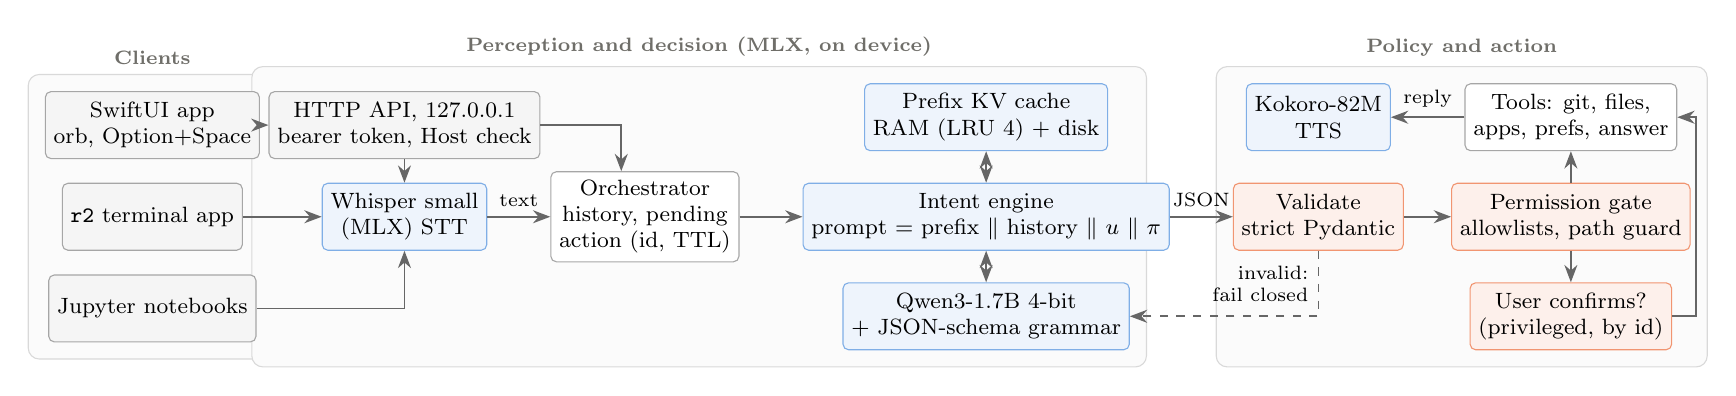
\begin{tikzpicture}[
  font=\footnotesize, >={Stealth[length=2.2mm]},
  box/.style={draw=black!35, rounded corners=2pt, fill=white, align=center, minimum height=8.5mm, inner sep=3pt},
  model/.style={box, fill=r2light, draw=r2blue!60},
  guard/.style={box, fill=r2orange!10, draw=r2orange!70},
  io/.style={box, fill=black!4},
  lane/.style={draw=black!15, rounded corners=4pt, fill=black!1.5, inner sep=6pt},
  arr/.style={->, draw=black!60, line width=0.6pt}]
  % clients
  \node[io] (app) {SwiftUI app\\ orb, Option+Space};
  \node[io, below=3mm of app] (cli) {\texttt{r2} terminal app};
  \node[io, below=3mm of cli] (nb) {Jupyter notebooks};
  % speech
  \node[model, right=10mm of cli] (stt) {Whisper small\\(MLX) STT};
  \node[io, above=3mm of stt] (http) {HTTP API, 127.0.0.1\\bearer token, Host check};
  % engine
  \node[box, right=8mm of stt] (orch) {Orchestrator\\history, pending\\action (id, TTL)};
  \node[model, right=8mm of orch] (engine) {Intent engine\\prompt $=$ prefix $\Vert$ history $\Vert$ $u$ $\Vert$ $\pi$};
  \node[model, above=4mm of engine] (kv) {Prefix KV cache\\RAM (LRU 4) + disk};
  \node[model, below=4mm of engine] (llm) {Qwen3-1.7B 4-bit\\+ JSON-schema grammar};
  % policy
  \node[guard, right=8mm of engine] (val) {Validate\\strict Pydantic};
  \node[guard, right=6mm of val] (gate) {Permission gate\\allowlists, path guard};
  \node[guard, below=4mm of gate] (conf) {User confirms?\\(privileged, by id)};
  \node[box, above=4mm of gate] (tools) {Tools: git, files,\\apps, prefs, answer};
  \node[model, above=4mm of val] (tts) {Kokoro-82M\\TTS};
  % arrows
  \draw[arr] (app) -- (http);
  \draw[arr] (http) -- (stt);
  \draw[arr] (http.east) -| ($(orch.north)+(-3mm,0)$);
  \draw[arr] (cli) -- (stt);
  \draw[arr] (nb.east) -| ($(stt.south)+(0,0)$);
  \draw[arr] (stt) -- node[above, font=\scriptsize]{text} (orch);
  \draw[arr] (orch) -- (engine);
  \draw[arr, <->] (kv) -- (engine);
  \draw[arr, <->] (engine) -- (llm);
  \draw[arr] (engine) -- node[above, font=\scriptsize]{JSON} (val);
  \draw[arr] (val) -- (gate);
  \draw[arr] (gate) -- (conf);
  \draw[arr] (gate) -- (tools);
  \draw[arr] (conf.east) -- ++(3mm,0) |- (tools.east);
  \draw[arr] (tools.west) -- node[above, font=\scriptsize]{reply} (tts.east);
  \draw[arr, dashed] (val.south) |- node[pos=0.25, left, font=\scriptsize, align=right]{invalid:\\fail closed} (llm.east);
  % lanes
  \begin{scope}[on background layer]
  \node[lane, fit=(app)(nb), label={[font=\scriptsize\bfseries, text=r2gray]above:Clients}] {};
  \node[lane, fit=(kv)(llm)(orch)(stt)(http), label={[font=\scriptsize\bfseries, text=r2gray]above:Perception and decision (MLX, on device)}] {};
  \node[lane, fit=(val)(gate)(conf)(tools)(tts), label={[font=\scriptsize\bfseries, text=r2gray]above:Policy and action}] {};
  \end{scope}
\end{tikzpicture}}
\caption{R2 architecture. Blue: learned models on MLX. Orange: deterministic policy that alone can
authorise execution. The LLM only proposes a JSON decision; invalid proposals fall back to a safe
heuristic, a clarifying question or a refusal.}
\label{fig:arch}
\end{figure*}

\subsection{Request lifecycle}

\Cref{alg:request} gives the per-request control flow. The orchestrator keeps the last three
user/assistant turns as compact JSON decisions rather than verbose tool output, which keeps the
prompt short and stable.

\begin{algorithm}[t]
\caption{Handling one request in R2}\label{alg:request}
\small
\begin{algorithmic}[1]
\Require utterance $u$ (typed, or Whisper transcript), history $h$
\Require confirmation id $c$ (empty unless the client is answering a prompt)
\If{a pending action $P$ exists}
  \If{$u\in\textsc{Yes}$} \State $P\gets$ \textsc{Take}$(P)$ \Comment{single use}
    \State \textbf{if} $P.\textsc{Check}(c)$ \textbf{then} \Return \textsc{Execute}$(P.d)$ via the gate
    \State \textbf{else} \Return ``Cancelled.'' \Comment{missing, wrong, expired, altered}
  \ElsIf{$u\in\textsc{No}$} \State drop $P$; \Return ``Cancelled.''
  \Else\ drop $P$ and handle $u$ as a new request
  \EndIf
\EndIf
\State $x \gets \mathrm{tokens}(\text{prefix}\,\Vert\,h\,\Vert\,u\,\Vert\,\pi)$
\State $(C, x_{\text{new}}) \gets \textsc{KV.acquire}(x)$ \Comment{reuse cached prefix}
\State $y \gets \textsc{Generate}(x_{\text{new}}, C, \text{mask}=A_G(\cdot), \text{greedy})$
\State \textsc{KV.release}$(C)$ \Comment{trim back to the prefix}
\State $d \gets \textsc{ParseJSON}(\pi\Vert y)$; $d\gets\textsc{Normalise}(d)$ \Comment{unknown keys: reject}
\If{$d$ invalid} \State retry once, else heuristic / clarify / unsupported \EndIf
\State $r \gets \textsc{Gate}(d)$, then the tool's precheck \Comment{allowlist, schema, path guard}
\If{$r$ denied} \Return refusal
\ElsIf{$r$ needs confirmation} \State $P\gets(d,\ \text{id},\ \text{TTL},\ \mathrm{sha256}(d))$
  \State \Return ``Open Safari? Say yes or no.'' and the id
\Else\ \Return $\textsc{Speak}(\textsc{Execute}(d))$
\EndIf
\end{algorithmic}
\end{algorithm}

\subsection{Prompt design}\label{sec:prompt}

The system prompt (\cref{fig:prompt}) contains 438 tokens of instructions---the JSON format, one
line per implemented intent with its parameter schema and \emph{when to use it}, the approved apps
and boundary rules---followed by 25 few-shot examples (675 tokens, 61\% of the prefix). The chat
template adds 5 tokens, giving the 1{,}118-token cached prefix. Qwen3's thinking mode is disabled
(\texttt{enable\_thinking=False}) because the task needs a label, not reasoning, and thinking tokens
would multiply latency.

\begin{figure}[t]
\centering
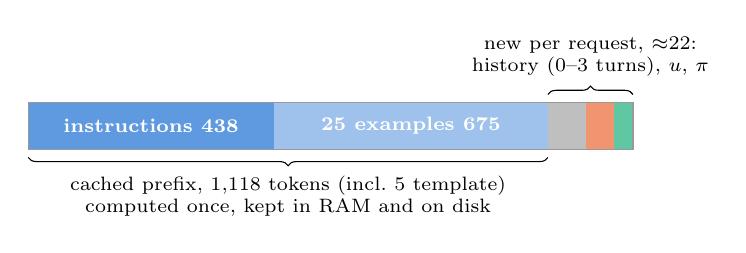
\begin{tikzpicture}[font=\scriptsize, x=0.6mm, y=1mm]
  \fill[r2blue!75] (0,0) rectangle (52,6);
  \fill[r2blue!45] (52,0) rectangle (110,6);
  \fill[black!25] (110,0) rectangle (118,6);
  \fill[r2orange!70] (118,0) rectangle (124,6);
  \fill[r2aqua!70] (124,0) rectangle (128,6);
  \draw[black!40] (0,0) rectangle (128,6);
  \node[white, font=\scriptsize\bfseries] at (26,3) {instructions 438};
  \node[white, font=\scriptsize\bfseries] at (81,3) {25 examples 675};
  \draw[decorate, decoration={brace, amplitude=3pt, mirror}] (0,-1) -- (110,-1)
     node[midway, below=3pt, align=center]{cached prefix, 1{,}118 tokens (incl.\ 5 template)\\computed once, kept in RAM and on disk};
  \draw[decorate, decoration={brace, amplitude=3pt}] (110,7) -- (128,7)
     node[midway, above=3pt, align=center]{new per request, $\approx$22:\\history (0--3 turns), $u$, $\pi$};
\end{tikzpicture}
\caption{Token layout of one request. Only the right-hand tokens (grey: history, orange: request, green: prefill $\pi$) are processed per request; after generation the cache is trimmed back to the prefix.}
\label{fig:prompt}
\end{figure}

\subsection{Clients and voice}

The SwiftUI client records audio with AVAudioEngine, uploads WAV to \texttt{/ask\_audio}, and plays
Kokoro speech from \texttt{/tts}, metering playback loudness at 60\,Hz to animate an orb. A global
\texttt{Option+Space} hot key, registered through Carbon's \texttt{RegisterEventHotKey}, summons R2
without Accessibility permissions. The terminal client offers push-to-talk and the same commands.
The app launches the core with \texttt{uv run r2 serve} and stops it on quit. On start it reads
the session token from a \texttt{0600} file and sends it with every request, rereading it once
after a 401 (the core rotates the token on every restart). It stores the confirmation id from a
prompt and attaches it both to the \emph{Confirm} button and to the next spoken utterance, so a
voice ``yes'' approves exactly the action that is on screen.

\subsection{Bounded multi-step requests}\label{sec:agent}

A request such as ``check git status and then find the Swift files'' becomes a \emph{plan} of at
most five ordinary decisions. The runtime adds sequencing but no new way to act: every step is
handed to the same executor (gate, validation, precheck, confirmation, tool), so deleting the
runtime would not change the set of reachable actions. The plan is made \emph{once}, before any
tool runs, by splitting the request on explicit connectors (``and then'', ``after that'', ``;'')
and routing each clause through the normal single-intent engine. A clause that routes to a tool
action and contains ``and'' or a comma is split further only if \emph{every} part also routes to a
tool action, and a request whose split would be rejected is routed once more as a whole, so that
``how do I rebase and then push?'' is answered as one question. Tool output is never fed back to a
planner, so a file that says ``now open Terminal'' cannot add a step, which is our main containment
of prompt injection. The whole plan is rejected if any step is invalid, unimplemented,
\texttt{unsupported} or \texttt{clarify\_request}. Privileged steps pause the run with the same
single-use, expiring confirmation id; the first failing step ends the run, and a wall-time budget
bounds it. Run history is stored as metadata only (intents, parameters, status, the short spoken
summary), never file contents or diffs. A one-shot model planner that emits the whole plan under a
grammar is available but not the default (\cref{sec:multistep}).

The app reaches runs through the ordinary \texttt{/ask} endpoint with an \texttt{allow\_runs}
flag: a request that plans to two or more steps starts a run, and the reply carries the run so
the client can draw one row per step. A paused run hands out its confirmation id exactly like a
single action, so the Confirm button, a typed ``yes'' and a spoken ``yes'' all continue it, and
a new request supersedes it. If any clause is refused, the reply is a refusal and nothing runs;
the client never falls back to executing the parts it understood. The Confirm button requires
Command--Return so that a stray Return can never approve a step.

% ================================================================ 6 Implementation
\section{Implementation}\label{sec:impl}

\subsection{Persistent prefix KV cache}

\Cref{lst:kv} shows the essential logic of \texttt{PrefixKVCache}. Three modes support
experiments: \texttt{none}, \texttt{prefix} (RAM) and \texttt{persistent} (RAM + disk). Several
prefixes---the intent prompt and the answer prompt---share an LRU of four entries in memory; on
disk, at most eight files are kept, evicted by least-recent use.

\begin{lstlisting}[caption={Acquire, release and fingerprinted persistence (abridged from \texttt{models/kv\_cache.py}).},label={lst:kv},float=t]
def fingerprint(**parts):  # revision, weights/tokenizer/config/adapter
    h = sha256(json.dumps(parts, sort_keys=True).encode())  # shas, template,
    return {**parts, "fingerprint": h.hexdigest()[:20]}     # mlx versions, prefix

def acquire(self, full_tokens):
    n = len(self._prefix_tokens)
    if (self._cache is None or len(full_tokens) <= n
            or full_tokens[:n] != self._prefix_tokens):
        return None, full_tokens, 0          # miss: full prefill
    return self._cache, full_tokens[n:], n   # hit: suffix only

def release(self, cache):                    # keep only the prefix
    extra = cache[0].offset - len(self._prefix_tokens)
    if extra > 0:
        trim_prompt_cache(cache, extra)

def _try_load(self, fp):
    cache, meta = load_prompt_cache(path, return_metadata=True)
    mx.eval([c.state for c in cache])        # loads are lazy
    if meta.get("fingerprint") != fp["fingerprint"]:
        return False                          # stale: rebuild
    return validate_layers(cache, self._layer_classes,
                           len(self._prefix_tokens)) is None

def _save(self, fp):                          # atomic, then evict LRU
    save_prompt_cache(tmp, self._cache, metadata=fp)
    os.replace(tmp, path)
\end{lstlisting}

Because \cref{cor:exact} requires an identical prefix at identical positions \emph{under identical
weights}, the fingerprint is derived from content rather than names. In the Hugging Face cache,
snapshot files are symbolic links to blobs named by the hash of their content (SHA-256 for weight
files)~\cite{hfcache2025}, so reading the link targets gives the identity of the weights, tokenizer
and configuration at no I/O cost. Files in a plain directory are hashed with SHA-256 up to 64\,MiB
and identified by size and modification time above that, which is weaker and documented as such.
The fingerprint also covers the snapshot revision, the adapter files, a hash of the chat template,
the mlx and mlx-lm versions and a hash of the prefix text; any change invalidates the file and
triggers a rebuild, which is what makes persistence safe. A matching fingerprint is not trusted on
its own: \texttt{validate\_layers} checks the number of layers and each layer's cache class
against the loaded model, and that \emph{every} layer's offset and key length equal the prefix
length. A truncated or mismatched file is therefore rebuilt rather than used. Files are written to
a temporary name and renamed into place, so a crash cannot leave a torn cache. The load is followed by \texttt{mx.eval} because MLX loads arrays lazily;
without it, load times would be under-reported. The token-level check in \texttt{acquire} also
guards against tokeniser merges across the prefix boundary: if the rendered prompt does not start
with exactly the cached tokens, R2 falls back to a full prefill.

\subsection{Constrained decoder}

\Cref{lst:mask} implements the allowed set of \cref{sec:constrained} as an mlx-lm logits processor.
The vocabulary strings and candidate list are cached at module level, so the cost is paid once per
process.

\begin{lstlisting}[caption={Intent-name mask (abridged from \texttt{models/constrained.py}).},label={lst:mask},float=t]
def allowed_ids(self, prefix):
    if prefix not in self._allowed_cache:
        self._allowed_cache[prefix] = [
            tid for tid, s in self._candidates
            if any(t.startswith(prefix + s) or (prefix + s).startswith(t)
                   for t in self.targets)]
    return self._allowed_cache[prefix]

def __call__(self, tokens, logits):
    if self.done:
        return logits
    text = self.tokenizer.decode(tokens[self.n_prompt:].tolist())
    if any(text.startswith(t) for t in self.targets):
        self.done = True                  # name complete
        return logits
    allowed = self.allowed_ids(text)
    if not allowed:                       # fail closed
        return eos_only(logits, self.eos)
    mask = np.full(logits.shape[-1], -np.inf, np.float32)
    mask[allowed] = 0.0
    return logits + mx.array(mask)
\end{lstlisting}

\paragraph{Schema grammar.}
In json mode (the default) the decision schema of \cref{sec:constrained} is generated from the
Pydantic parameter models of the implemented intents and compiled by
llguidance~\cite{llguidance2025} with the separators used in the few-shot examples
(\texttt{", "} and \texttt{": "}) and no free whitespace, so the grammar and the prompt agree on
one canonical form. The compiled matcher is cached per tokenizer and schema and copied for each
request. Per step the processor feeds new tokens to the matcher, fills a token bitmask on the CPU
and applies it to the logits with a Metal kernel; a rejected token, a matcher error or an empty
mask leaves only end-of-sequence. If json mode is configured but llguidance is missing, R2 refuses
to start rather than silently falling back to a weaker mode.

\subsection{Validation, normalisation and safety}\label{sec:safety}

Model output passes four deterministic stages before anything executes.
\begin{enumerate}
\item \textbf{Parsing:} the first complete JSON object is extracted with a non-greedy decoder.
\item \textbf{Normalisation:} unknown parameter keys are \emph{rejected}, which sends the request
  to the retry and fallback path (an earlier version silently dropped them), and search terms are
  mapped to globs, e.g.\ \texttt{swift}, \texttt{*swift*} or ``swift files'' $\to$
  \texttt{*.swift}, while \texttt{config} $\to$ \texttt{*config*}.
\item \textbf{Validation:} a Pydantic model per intent rejects missing or extra fields and
  over-long values.
\item \textbf{Authorisation:} the permission gate checks the intent is implemented and enabled,
  apps are on the allowlist, and paths resolve inside the workspace. A tool-specific precheck
  (for example the app allowlist) runs \emph{before} any confirmation is requested, so the user is
  never asked to approve an action that would be refused anyway.
\end{enumerate}
Formally, a decision $d$ executes only when
\begin{multline}
\mathrm{Exec}(d)\iff\mathrm{Valid}(d)\wedge\mathrm{Allowed}(d)\wedge\mathrm{InWorkspace}(d)\\
\wedge\big(\neg\mathrm{Priv}(d)\vee\mathrm{Confirm}_{\text{user}}(d)\big),
\end{multline}
where $\mathrm{Confirm}_{\text{user}}$ can only come from a later user turn, never from model text.
It is also bound to the prompt the user saw: a pending action carries a random single-use id, a
time-to-live (120\,s) and a SHA-256 digest of the decision, and a ``yes'' approves it only if the id
matches, the action has not expired and the digest is unchanged. Any other attempt cancels the
action, and execution re-runs the gate. In-process clients (terminal, notebooks) show the prompt
in the same process and do not need the id.
Every failure path is closed: a parse error triggers one retry and then a heuristic classifier
whose outputs are themselves validated; reading files refuses secrets (\texttt{.env*},
\texttt{*.pem}, \texttt{*.key}, \texttt{.netrc}); and \texttt{answer\_question} produces text that
is displayed and spoken but never executed. There is no shell tool.

\paragraph{File tools.}
Path checks on names alone are vulnerable to symbolic links and to a change between check and use.
\texttt{read\_file} opens with \texttt{O\_NOFOLLOW}, refuses anything that is not a regular file
(so a FIFO cannot block it), and re-checks the real path of the \emph{opened descriptor}
(\texttt{F\_GETPATH} on macOS) against the workspace and the secret-file rules before reading.
\texttt{search\_files} walks the tree without following directory links, skips links that leave
the workspace, and replaces control characters in file names so a crafted name cannot spoof the
spoken or displayed output. Adversarial tests cover links to outside files, a link named
\texttt{notes.txt} that points at \texttt{.env}, both race orders, FIFOs and spoofed names.

\paragraph{Local HTTP API.}\label{sec:api}
A loopback-only server is still reachable by any web page the user visits, and by DNS rebinding.
Following the guidance for local MCP servers~\cite{mcpsecurity2025}, every request must carry a
\texttt{Host} of \texttt{127.0.0.1}, \texttt{localhost} or \texttt{[::1]} on the bound port;
requests with an \texttt{Origin} header or \texttt{Sec-Fetch-Site: cross-site} are refused; bodies
must be JSON (or WAV for audio), which forces a CORS preflight that the server never grants; and
every route except \texttt{/health} needs a bearer token. The token is random, rotated on every
start, written atomically to a \texttt{0600} file and removed on shutdown. Browsers are also
adding permission prompts for requests to local addresses~\cite{chromelna2025}, but R2 does not
depend on them. The boundary is deliberately the user account: a process running as the same user
can read the token, as it can read the preference database and the configuration. The token stops
browsers, other users and accidental clients, not malware the user is already running.

\subsection{Software}

The core is Python 3.12 (managed by \texttt{uv}) with mlx 0.32.4, mlx-lm 0.32.2, mlx-whisper 0.4.3,
mlx-audio 0.6.3, llguidance 1.9.1 and Pydantic 2.14; the client is SwiftUI (Swift 6.3,
macOS 14+). 195 unit, integration and adversarial tests run without model downloads, a
microphone or network access.

% ================================================================ 7 Setup
\section{Experimental Setup}\label{sec:setup}

\paragraph{Hardware and model.}
All measurements use an Apple M4 (4 performance and 6 efficiency CPU cores, 8-core GPU) with
16\,GB of unified memory and a nominal 120\,GB/s memory bandwidth, on macOS 26.5. The model is
\texttt{mlx-community/Qwen3-1.7B-4bit} (\cref{tab:model}). Decoding is greedy (temperature 0) with
at most 128 new tokens.

\begin{table}[t]
\centering\small
\caption{Model configuration (Qwen3-1.7B, MLX 4-bit).}
\label{tab:model}
\begin{tabular}{@{}lr@{\hspace{1.5em}}lr@{}}
\toprule
Layers $L$ & 28 & Hidden size $d$ & 2{,}048 \\
Query heads $H$ & 16 & KV heads $\Hkv$ & 8 \\
Head dim $d_h$ & 128 & FFN size & 6{,}144 \\
Vocabulary & 151{,}936 & Weights & 4-bit, group 64 \\
Weight file & 0.94\,GB & KV / token & 112\,KiB \\
\bottomrule
\end{tabular}
\end{table}

\paragraph{Datasets.}
The \emph{dev set} (\texttt{eval\_heldout.jsonl}, 40 cases) covers ten intents and was used while
designing the prompt. The \emph{fresh test set} (\texttt{eval\_fresh.jsonl}, 24 cases, all eleven
intents) was written \emph{before} the final round of prompt changes and never used to tune them;
we report it both before and after that round. Neither set overlaps the few-shot examples.

\paragraph{Metrics.}
\emph{Intent accuracy} is exact match of the intent. \emph{Parameter accuracy} additionally
requires the normalised required parameters to match. \emph{Malformed rate} counts outputs that do
not parse into a valid decision; \emph{fallback rate} counts requests answered by the heuristic.
TTFT is measured from the start of generation to the first token; \emph{decision latency} covers
prompt rendering, generation, parsing and validation. For proportions we report 95\% Wilson score
intervals.

\paragraph{Benchmarks.}
\texttt{bench\_kv.py} runs 20 dev utterances end-to-end in each cache mode.
\texttt{bench\_scaling.py} isolates the model: for prefix lengths $n$ from 128 to 8{,}192 tokens
(R2's real prompt, repeated as needed) and a 22-token suffix it times an uncached forward pass over
$n+s$ tokens, a cached forward pass over $s$ tokens, one decode step, KV size, and safetensors
save/load, reporting the median of 3 runs after warm-up. \texttt{bench\_voice.py} times Whisper on
8 synthetic utterances and Kokoro on 4 replies.

% ================================================================ 8 Results
\section{Results}\label{sec:results}

\subsection{End-to-end cache modes}

\begin{figure*}[t]
\centering
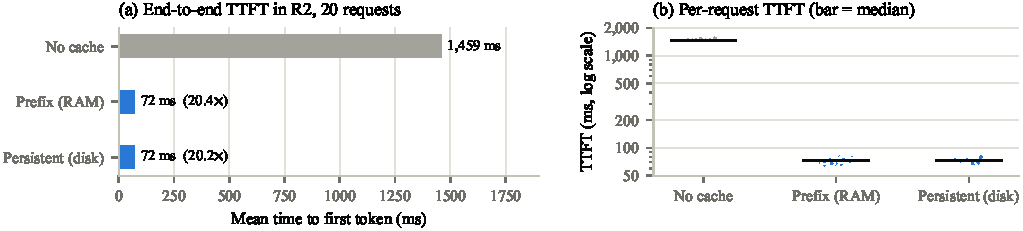
\includegraphics[width=\textwidth]{figures/kv_modes.pdf}
\caption{End-to-end TTFT inside R2 for 20 dev requests. Both cached modes reach about 71--75\,ms;
the spread across requests is small because only the short suffix varies.}
\label{fig:kvmodes}
\end{figure*}

\begin{table}[t]
\centering\small
\caption{End-to-end cache modes, 20 requests (mean $\pm$ s.d.).}
\label{tab:kvmodes}
\setlength{\tabcolsep}{3.5pt}
\begin{tabular}{@{}lrrrr@{}}
\toprule
Mode & Setup & Prefilled & TTFT (ms) & Decision (ms) \\
\midrule
None & -- & 1{,}140 & $1459\pm38$ & $1611\pm74$ \\
Prefix (RAM) & 1.52\,s build & 22 & $\mathbf{72\pm4}$ & $227\pm46$ \\
Persistent & 82\,ms load & 22 & $\mathbf{72\pm3}$ & $229\pm45$ \\
\bottomrule
\end{tabular}
\end{table}

\Cref{tab:kvmodes,fig:kvmodes} show the effect inside the running assistant. Prefix caching cuts
mean TTFT from 1{,}459\,ms to 72\,ms, a 20.4$\times$ speed-up, and whole decisions from 1.61\,s to
0.23\,s. The persistent mode matches the in-memory mode while replacing a 1.52\,s rebuild
with an 82\,ms load at start-up (18.5$\times$ faster readiness). The measured speed-up is below the
token-ratio bound of 51.8 (\cref{eq:bound}) because of the fixed per-pass cost and request work
outside the model, quantified next.

\subsection{Scaling with context length}

\begin{figure*}[t]
\centering
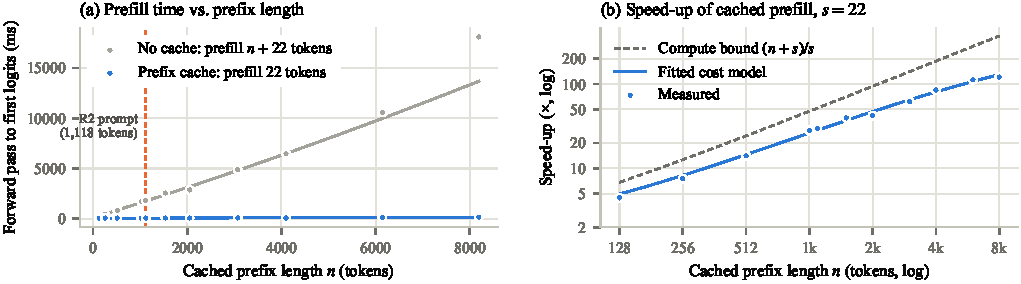
\includegraphics[width=\textwidth]{figures/scaling.pdf}
\caption{(a) Forward-pass time to the first logits for an uncached prompt of $n+22$ tokens and for
22 tokens on top of an $n$-token cached prefix; lines are the fitted models of
\cref{eq:tpre,eq:tsuf}. (b) The resulting speed-up against the compute bound $(n+s)/s$; the gap is
the fixed cost $\alpha$ of a forward pass.}
\label{fig:scaling}
\end{figure*}

\begin{table}[t]
\centering\small
\caption{Model-only sweep, $s=22$ (median of 5). KV is the allocated size; $\Delta z$ is the
largest absolute logit difference between cached and uncached runs.}
\label{tab:scaling}
\setlength{\tabcolsep}{3pt}
\begin{tabular}{@{}rrrrrrr@{}}
\toprule
$n$ & Uncached & Cached & $S$ & Decode & KV & $\max|\Delta z|$ \\
 & (ms) & (ms) & & (ms) & (MiB) & \\
\midrule
128 & 244 & 54.5 & 4.5 & 12.7 & 28 & 0.47 \\
256 & 428 & 56.7 & 7.6 & 12.4 & 28 & 0.38 \\
512 & 824 & 58.3 & 14.1 & 13.8 & 56 & 0.31 \\
1{,}024 & 1{,}698 & 60.3 & 28.1 & 14.4 & 112 & 0.50 \\
\textbf{1{,}118} & \textbf{1{,}813} & \textbf{60.7} & \textbf{29.8} & 12.7 & 140 & 0.44 \\
1{,}536 & 2{,}554 & 64.2 & 39.8 & 16.5 & 168 & 0.44 \\
2{,}048 & 2{,}870 & 68.0 & 42.2 & 16.3 & 224 & 0.00 \\
3{,}072 & 4{,}887 & 79.2 & 61.7 & 17.3 & 336 & 0.28 \\
4{,}096 & 6{,}478 & 76.2 & 85.0 & 18.1 & 448 & 0.00 \\
6{,}144 & 10{,}580 & 93.9 & 112.7 & 21.6 & 672 & 0.00 \\
8{,}192 & 18{,}106 & 149.6 & 121.0 & 24.9 & 896 & 0.00 \\
\bottomrule
\end{tabular}
\end{table}

\Cref{tab:scaling,fig:scaling} isolate the model. Uncached prefill grows almost linearly, from
244\,ms at 128 tokens to 6.5\,s at 4{,}096, while the cached 22-token pass stays between 55 and
80\,ms. Least-squares fits over 128--4{,}096 tokens give
\begin{align}
T_{\text{pre}}(N)&=55.4+1.460\,N+2.43{\times}10^{-5}N^2\ \text{ms}\quad(R^2=0.996),\\
T_{\text{suf}}(22\mid n)&=54.7+0.00621\,n\ \text{ms}\quad(R^2=0.920).
\end{align}
These coefficients agree with \cref{eq:tpre}. Counting $P\approx1.72$B parameters per token
(1.41B in the transformer blocks plus the 0.31B tied output head), the linear coefficient implies
an effective throughput $\Pi=2P/b\approx2.4$\,TFLOP/s. At that throughput \cref{eq:tpre}
predicts $c=2LHd_h/\Pi=4.9{\times}10^{-5}$\,ms/token$^2$, within a factor of two of the fitted
$2.4{\times}10^{-5}$ (the quadratic term is small and poorly determined below 4k tokens). The crossover length $N^\star=b/c\approx60{,}000$ tokens confirms that R2
operates deep in the linear, weight-bound regime, where the speed-up approaches the token ratio
minus overhead. At R2's prompt length the model-only speed-up is 29.8$\times$; the end-to-end
20.4$\times$ of \cref{tab:kvmodes} additionally includes about 11\,ms of tokenisation, sampling and
masking per request. Beyond the fitted range the sweep reaches 121$\times$ at 8{,}192 tokens, but
uncached prefill there (18.1\,s) is 32\% above the extrapolated fit and the cached pass jumps to
150\,ms: at 6--8k tokens the 16\,GB machine leaves the clean weight-bound regime.

\subsection{Memory, decode and disk}

\begin{figure*}[t]
\centering
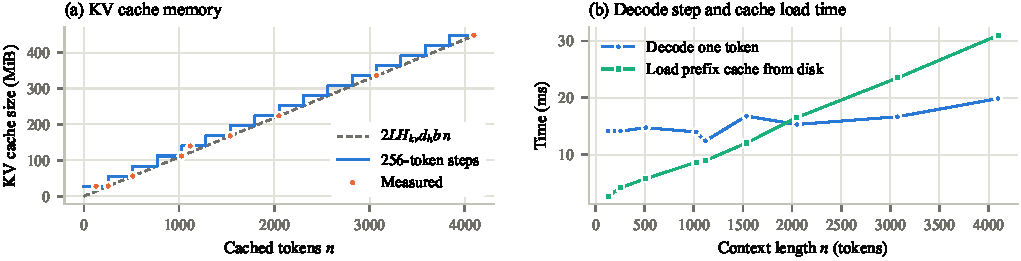
\includegraphics[width=\textwidth]{figures/memory.pdf}
\caption{(a) Measured KV size (dots) matches \cref{eq:alloc} exactly, including the 256-token
allocation steps. (b) Decode time per token rises slowly with context; loading a prefix cache that
is already in the OS page cache takes 2.5--57\,ms.}
\label{fig:memory}
\end{figure*}

\Cref{fig:memory}a confirms \cref{eq:mem,eq:alloc} to the byte: every measured cache size equals
$114{,}688\cdot256\lceil n/256\rceil$ bytes. Decoding (\cref{fig:memory}b) costs
$12.6+0.00149\,n$\,ms per token. Reading the 0.94\,GB of weights in 12.6\,ms implies an achieved
bandwidth of about 74\,GB/s (62\% of nominal), and at that bandwidth \cref{eq:tdec} predicts a
per-context-token slope of $114{,}688/74\text{\,GB/s}=0.0015$\,ms, matching the fitted 0.00149. The
end-to-end generation rate is about 77 tokens/s (median), and R2's peak memory during evaluation is
1.36\,GB.

Disk loading is fast when the file is in the page cache (8\,ms for R2's 140\,MiB at 1{,}118 tokens,
about 17\,GB/s), and 82\,ms on a cold start of the assistant, which includes reading from SSD,
parsing safetensors metadata and verifying the fingerprint. Both are far below the 1.5--1.7\,s cost
of rebuilding the prefix.

\subsection{Numerical equivalence}\label{sec:equiv}

In exact arithmetic \cref{cor:exact} guarantees identical logits. In bfloat16 the cached and
uncached computations use different kernel shapes, so the largest absolute logit difference at the
last position ranges from 0 to 0.5 (\cref{tab:scaling}), while the argmax token is identical at all
nine lengths. End-to-end, greedy outputs with and without the cache were identical in 20 of 20
requests in both cached modes. Caching therefore changes latency, not behaviour.

\subsection{Conversation-level reuse}\label{sec:convreuse}

\begin{table}[t]
\centering\small
\caption{Multi-turn routing (\emph{new in revision 2}): 10 sessions $\times$ 10 held-out requests,
history $\le$3 turns, all five configurations interleaved per session in rotated order. Absolute
times are higher than in \cref{tab:kvmodes} because of background load during the run; compare
rows. Pref.: tokens prefilled per turn. Exact: decision vs.\ the single-turn label.}
\label{tab:convreuse}
\setlength{\tabcolsep}{2.6pt}
\begin{tabular}{@{}lrrrrr@{}}
\toprule
History / cache & TTFT & Turns 1--4 & Turns 5+ & Pref. & Exact \\
\midrule
None / prefix & 96 & 96 & 95 & 21 & 92 \\
Sliding / prefix (default) & 254 & 192 & 295 & 103 & 90 \\
Sliding / + conversation & 235 & 138 & 300 & 87 & 90 \\
Block / prefix & 208 & 181 & 227 & 82 & 87 \\
Block / + conversation & \textbf{147} & 136 & \textbf{154} & 42 & 87 \\
\bottomrule
\end{tabular}
\end{table}

The prefix cache stops at the system prompt, so a request with three turns of history still
prefills about 100 tokens and its TTFT roughly triples. R2 can therefore keep the KV state of each
routing prompt and, on the next turn, reuse the longest token prefix it shares with a stored one.
The store is mlx-lm's \texttt{LRUPromptCache}, a token trie that hands out copies, which are cheap
because MLX arrays are copy-on-write (about 3\,ms per turn). Generated tokens are trimmed off before
storing, because Qwen3 renders earlier assistant turns without the empty think block, so each turn
still prefills the previous reply and the new request. Only live conversation turns are stored;
planner clauses, evaluation and warm-up are not, so they cannot evict the entry.

\Cref{tab:convreuse} gives three results. First, reuse does not change behaviour: all 100 intents
and graded parameters were identical with and without it, and the only differences were free-text
refusal reasons (3 and 2 of 100), as \cref{sec:equiv} predicts. Second, with R2's sliding
window, reuse helps only while history grows (turns 2--4, $-28\%$). Once the window is full,
the oldest turn is dropped and every later token shifts position. Nothing beyond the system prefix
then matches, and turns 5+ are unchanged. Third, a \emph{block} window, which keeps only the latest
turn when the window overflows, keeps the prefix stable and gives a flat $\approx$150\,ms
($-42\%$ overall, $-48\%$ after turn 4). The shorter history, however, cost 3 of 100 exact
decisions, among them ``make it better'' routed to a (confirmation-gated)
\texttt{remember\_preference}. Without any history, routing is 2.7$\times$ faster than the default
and no less accurate on these single-turn labels. The benefit of history for follow-ups (``open
it'', ``why did that fail?'') is not measured by this set. Conversation reuse therefore ships
\emph{off} by default (one stored entry costs 147\,MB), and the history policy, not the cache, is the
larger lever.

\begin{figure}[t]
\centering
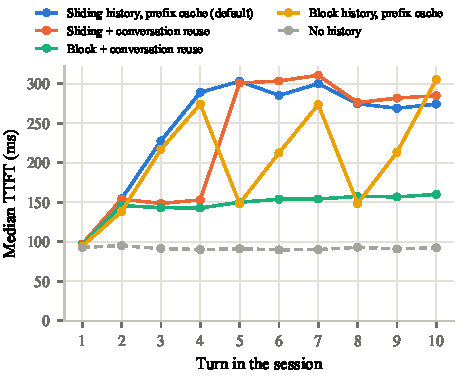
\includegraphics[width=\columnwidth]{figures/conversation.pdf}
\caption{Median TTFT by turn (10 sessions). Reuse follows the history: with a sliding window it
stops after turn 4; a block window keeps it flat.}
\label{fig:conversation}
\end{figure}

\subsection{Quantised KV and rotating windows}\label{sec:kvvariants}

\begin{figure*}[t]
\centering
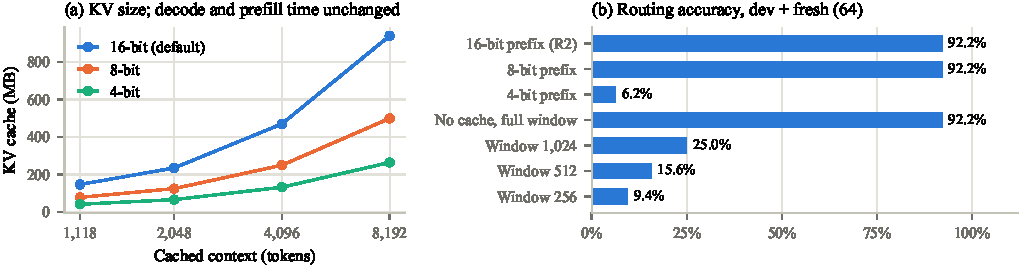
\includegraphics[width=\textwidth]{figures/kv_variants.pdf}
\caption{(a) KV size by context length and precision; it follows \cref{eq:memq} exactly.
(b) Exact routing accuracy on dev + fresh (64 requests) for quantised prefix caches and for
rotating windows shorter than R2's 1.1k-token prompt.}
\label{fig:kvvariants}
\end{figure*}

\begin{table}[t]
\centering\small
\caption{KV precision at four context lengths (\emph{new in revision 2}): cached size, 22-token
cached forward, one decode step, and the last-position logits against 16-bit.}
\label{tab:kvquant}
\setlength{\tabcolsep}{2.6pt}
\begin{tabular}{@{}rrrrrrr@{}}
\toprule
$n$ & Bits & MB & Fwd (ms) & Dec (ms) & max$|\Delta z|$ & KL \\
\midrule
1{,}118 & 16 & 146.8 & 57.4 & 15.3 & -- & -- \\
 & 8 & 78.0 & 56.2 & 13.2 & 1.1 & $10^{-8}$ \\
 & 4 & 41.3 & 56.2 & 13.3 & 48.5 & 25.8 \\
4{,}096 & 16 & 469.8 & 69.2 & 18.7 & -- & -- \\
 & 8 & 249.6 & 73.5 & 19.3 & 1.0 & $<10^{-8}$ \\
 & 4 & 132.1 & 73.1 & 18.5 & 39.2 & 6.7 \\
8{,}192 & 16 & 939.5 & 87.9 & 23.1 & -- & -- \\
 & 8 & 499.1 & 92.1 & 23.4 & 1.1 & $<10^{-9}$ \\
 & 4 & 264.2 & 100.7 & 21.0 & 37.1 & 0.23 \\
\bottomrule
\end{tabular}
\end{table}

\texttt{model.kv\_bits} quantises the prefix cache once after it is built (affine, groups of 64);
request tokens are then appended quantised. The disk fingerprint includes the bit width, and
\texttt{kv\_bits} cannot be combined with a rotating window, which mlx-lm cannot quantise.
\Cref{tab:kvquant,fig:kvvariants} give three results. (i) 8-bit KV halves the cache exactly as
\cref{eq:memq} predicts, keeps the logits within 1.1 of 16-bit at every length (argmax and top-5
unchanged), and routes the 64 requests with the same 92.2\% exact accuracy (two intents flipped,
one in each direction). (ii) It brings no speed-up: forward and decode times are within noise up to
8k tokens, as the cost model predicts when the weights dominate the bytes read, and dequantisation
adds work. (iii) 4-bit KV breaks Qwen3: at R2's own prompt length the last-position argmax changes
(KL 25.8) and routing collapses to 6.2\%. Rotating windows ($W=1{,}024$, 512, 256 with 4 sink tokens)
drop most of the instructions (\cref{cor:lcp}) and route only 25.0, 15.6 and 9.4\% correctly, with
no speed benefit since nothing is cached. Because R2's history is bounded, its context never
outgrows memory, so neither technique is enabled by default; 8-bit KV is available for longer
contexts.

\subsection{Accuracy}

\begin{figure}[t]
\centering
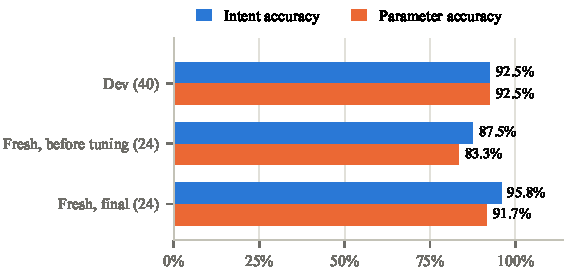
\includegraphics[width=\columnwidth]{figures/accuracy.pdf}
\caption{Intent and parameter accuracy on the dev set, on the fresh set before and after the final
prompt revision, and on the test set written later (default configuration).}
\label{fig:accuracy}
\end{figure}

\begin{table}[t]
\centering\small
\caption{Accuracy with 95\% Wilson intervals. All runs: 0\% malformed, 0\% fallback.}
\label{tab:accuracy}
\setlength{\tabcolsep}{3pt}
\begin{tabular}{@{}lrll@{}}
\toprule
Set & $n$ & Intent acc. & Param.\ acc. \\
\midrule
Dev & 40 & 92.5 [80.1, 97.4] & 92.5 [80.1, 97.4] \\
Fresh, before revision & 24 & 87.5 [69.0, 95.7] & 83.3 [64.1, 93.3] \\
Fresh, final & 24 & \textbf{95.8} [79.8, 99.3] & \textbf{91.7} [74.2, 97.7] \\
Test & 60 & 85.0 [73.9, 91.9] & 85.0 [73.9, 91.9] \\
\bottomrule
\end{tabular}
\end{table}

\Cref{tab:accuracy,fig:accuracy} report accuracy with the default configuration (schema grammar,
strict validation). On the fresh set R2 chooses the right intent for 23 of 24 requests and the right
parameters for 22. The prompt revision that sharpened the boundaries between \texttt{general\_help},
\texttt{answer\_question}, \texttt{clarify\_request} and \texttt{unsupported} raised fresh-set intent
accuracy from 87.5\% to 95.8\%; because the fresh set predates the revision, this is evidence of
generalisation, although the intervals are wide. The \emph{test} set (\emph{new in revision 2},
60 requests) was written later, before any LoRA training data, and deliberately targets weak spots
found during development: Dockerfiles and dotfiles, git write commands, vague requests and recalled
preferences. R2 gets 85.0\% of it exactly right; its nine errors are analysed in
\cref{sec:errors}. Median decision latency is 267\,ms on dev and fresh (90th percentile
354 and 350\,ms) and 303\,ms on the test set (\cref{fig:latency}).

\begin{figure}[t]
\centering
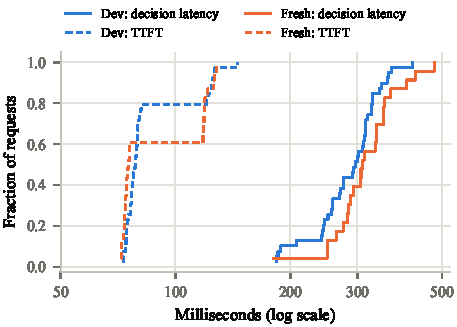
\includegraphics[width=\columnwidth]{figures/latency.pdf}
\caption{Cumulative distribution of TTFT and decision latency over the dev, fresh and test sets (the
first request, which includes GPU kernel compilation, is excluded).}
\label{fig:latency}
\end{figure}

\subsection{Ablation: few-shot examples vs.\ constrained decoding}\label{sec:ablation}

\begin{figure}[t]
\centering
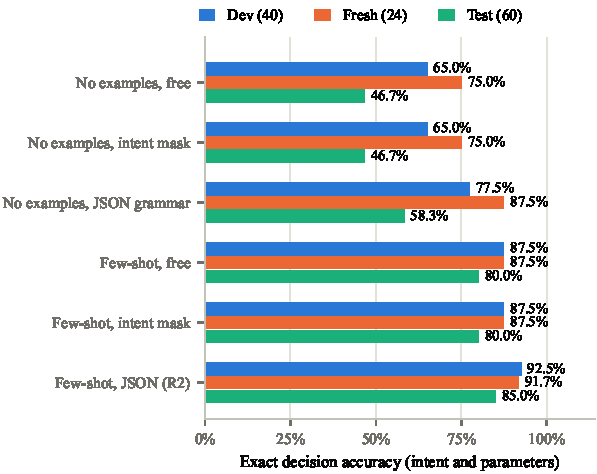
\includegraphics[width=\columnwidth]{figures/ablation.pdf}
\caption{Exact decision accuracy (intent and parameters) for few-shot examples on/off and three
decode constraints, under strict validation, on all three sets.}
\label{fig:ablation}
\end{figure}

\begin{table}[t]
\centering\small
\caption{Few-shot examples (FS) $\times$ decode constraint under \emph{strict} validation (unknown
keys rejected). Exact accuracy in \%; fallback rate and median decision latency on the test set.}
\label{tab:ablation3}
\setlength{\tabcolsep}{3.2pt}
\begin{tabular}{@{}clrrrr@{}}
\toprule
FS & Constraint & Dev (40) & Fresh (24) & Test (60) & Fallb. / ms \\
\midrule
 & none & 65.0 & 75.0 & 46.7 & 20.0 / 404 \\
 & intent & 65.0 & 75.0 & 46.7 & 20.0 / 381 \\
 & json & 77.5 & 87.5 & 58.3 & 0.0 / 240 \\
\checkmark & none & 87.5 & 87.5 & 80.0 & 6.7 / 332 \\
\checkmark & intent & 87.5 & 87.5 & 80.0 & 6.7 / 344 \\
\checkmark & \textbf{json} & \textbf{92.5} & \textbf{91.7} & \textbf{85.0} & \textbf{0.0} / 323 \\
\bottomrule
\end{tabular}
\end{table}

\Cref{tab:ablation3,fig:ablation} separate the techniques (\emph{re-measured in revision 2} on all
three sets). The 25 few-shot examples are the largest single gain: with free decoding they raise
exact accuracy from 65.0 to 87.5\% on dev and from 46.7 to 80.0\% on the test set. Their cost is
prompt length (675 of 1{,}118 tokens), which is exactly what the prefix cache makes free: without
caching, few-shot prompting would add roughly 0.9\,s to every request (\cref{eq:tpre}). The
intent-name mask changes nothing on any set. It governs only the intent \emph{name}, and every
error it could prevent is a parameter error; its value is a guarantee that no output names a
non-existent action.

\paragraph{Strict validation and the schema grammar.}
Dropping unknown parameter keys hides model errors, so the parser rejects them. The model often
adds a stray parameter, such as \texttt{git\_status \{"clean": \dots\}}; rejected outputs go to the
heuristic fallback (5--7\% of requests with examples, 15--20\% without). Constraining decoding to the
full decision schema makes such outputs impossible to generate: fallbacks drop to zero on every set
and exact accuracy rises by 5 points on dev and test, at no latency cost (decode stays at
12.8--13.9\,ms per token in every mode, because the mask is computed on the CPU in tens of
microseconds). Without examples the grammar adds 11.6--12.5 points. The sets are small (one case is
2.5, 4.2 and 1.7 points), so individual differences are indicative rather than significant, but the
ranking is the same on all three sets.

\subsection{Multi-step planning}\label{sec:multistep}

\begin{table}[t]
\centering\small
\caption{Planners on multi-step requests (plans validated, not executed). Fresh: 30 requests
written before the and-split and question guard existed. Rej.: share of must-refuse requests
refused.}
\label{tab:multistep}
\setlength{\tabcolsep}{3pt}
\begin{tabular}{@{}lrrrr@{}}
\toprule
Planner & Dev (61) & Fresh (30) [95\% CI] & Rej. & p50 \\
\midrule
Clause & 75.4 & 66.7 [48.8, 80.8] & 100 & 607\,ms \\
Clause + and-split + guard & \textbf{93.4} & \textbf{93.3} [78.7, 98.2] & 100 & 910\,ms \\
Model (one shot) & 47.5 & 40.0 [24.6, 57.7] & 0 & 396\,ms \\
\bottomrule
\end{tabular}
\end{table}

\Cref{tab:multistep} compares planners on a dev set of 61 multi-step requests (connectors, a bare
``and'', three to five steps, single questions that contain ``and then'', and requests with a
destructive or out-of-scope part that must be refused) and on a fresh set of 30 written before the
clause planner's options were implemented. The options raise exact-plan accuracy on the fresh set
from 66.7\% to 93.3\% while still refusing every must-refuse request; the price is about 300\,ms of
extra routing calls (fresh-set medians, re-measured). The one-shot model planner is faster but produces well-formed, wrong plans that
no validator can catch: it drops steps, copies few-shot parameters, and, most importantly,
\emph{silently omits} the part of a request it should refuse (``show me the diff then change it''
becomes just the diff) instead of rejecting the plan. The clause planner's remaining errors are
single-intent routing mistakes, such as ``commit everything'' routed to \texttt{git\_status}.

\subsection{Error analysis}\label{sec:errors}

\begin{figure}[t]
\centering
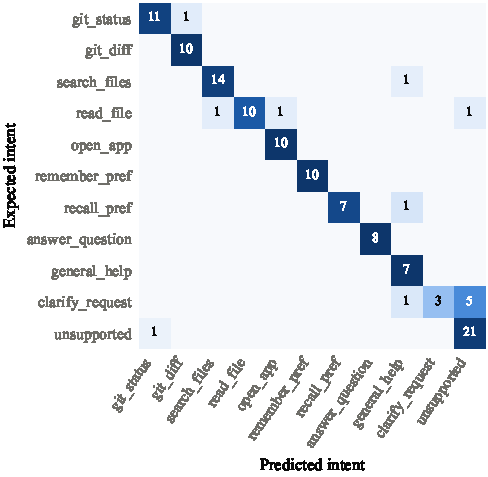
\includegraphics[width=0.92\columnwidth]{figures/confusion.pdf}
\caption{Confusion matrix over the dev, fresh and test sets (124 cases), default configuration.}
\label{fig:confusion}
\end{figure}

\begin{figure}[t]
\centering
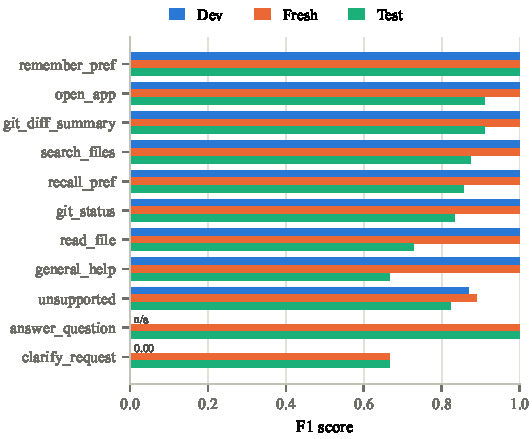
\includegraphics[width=\columnwidth]{figures/f1.pdf}
\caption{Per-intent F1 on the three sets. \texttt{answer\_question} does not occur in the dev set.}
\label{fig:f1}
\end{figure}

On dev and fresh, all four intent errors (\cref{fig:confusion,fig:f1}) share one pattern: vague commands such as
``do the thing'', ``make it better'', ``check that'' and ``change that thing'' are classified as
\texttt{unsupported}, often with the reason ``destructive actions are not allowed'', instead of
prompting a clarifying question. The model conflates \emph{unclear} with \emph{unsafe}. This failure
is benign, because a refusal executes nothing, but it is the main remaining accuracy gap. The single
parameter error maps ``list the yaml files'' to \texttt{*.yml} rather than \texttt{*.yaml}, a
defensible reading that an extension-alias table would resolve. During development we also found and
fixed a normalisation bug in which \texttt{*swift*} matched compiler caches under \texttt{.build/};
file search now skips build directories.

The nine test-set errors are more varied, which is what the set was written to expose. Two are
again vague commands refused or answered with help (``clean this up'', ``do it again but better'').
Three are file requests the router does not recognise as files: ``print the Dockerfile'' (refused),
``what's in .gitignore'' (searched instead of read) and ``open src/narrow\_ai/settings.py'' (routed
to \texttt{open\_app} Finder, which the gate would then refuse). ``Are there any dockerfiles'' becomes
\texttt{general\_help}, ``which files are modified'' becomes a diff summary instead of status, ``what
indentation do I prefer'' becomes help instead of recall, and ``commit everything'' is routed to
\texttt{git\_status} instead of being refused. None of these errors executes anything outside the
policy, since the substituted actions are read-only or refused by the gate, but they set the target
for fine-tuning (\cref{sec:lora}).

\subsection{LoRA fine-tuning}\label{sec:lora}

\begin{figure*}[t]
\centering
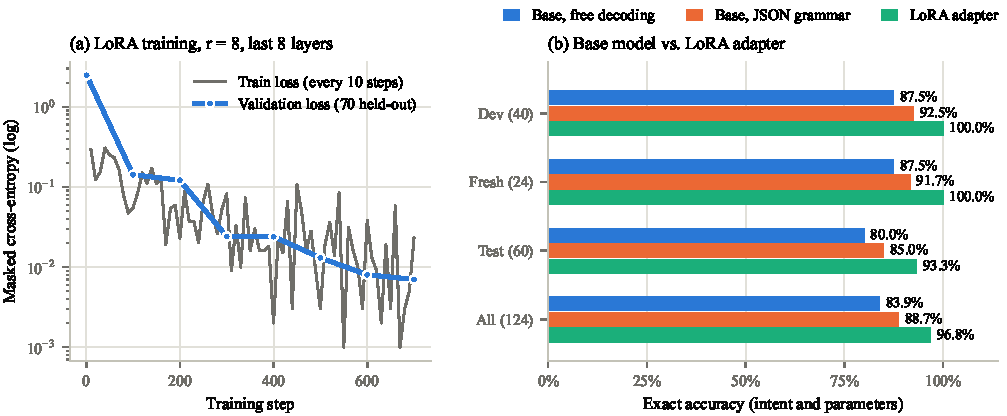
\includegraphics[width=\textwidth]{figures/lora.pdf}
\caption{(a) Loss on the decision tokens only, for training (every 10 steps) and the 70-example
validation split. (b) Exact accuracy of the base model with and without the JSON grammar and of
the LoRA adapter (grammar on; without it the adapter's numbers are identical).}
\label{fig:lora}
\end{figure*}

\begin{table}[t]
\centering\small
\caption{Base model vs.\ LoRA adapter, exact accuracy (\%) with the R2 prompt. Pooled: all 124
requests, Wilson 95\% interval. $p$: exact two-sided McNemar test~\cite{mcnemar1947note} on paired outcomes
(adapter vs.\ base, same constraint, pooled).}
\label{tab:lora}
\setlength{\tabcolsep}{3pt}
\begin{tabular}{@{}llrrrrr@{}}
\toprule
Model & Constr. & Dev & Fresh & Test & Pooled [95\% CI] & $p$ \\
\midrule
Base & json & 92.5 & 91.7 & 85.0 & 88.7 [81.9, 93.2] & -- \\
Base & none & 87.5 & 87.5 & 80.0 & 83.9 [76.4, 89.3] & -- \\
LoRA & json & \textbf{100} & \textbf{100} & \textbf{93.3} & \textbf{96.8} [92.0, 98.7] & 0.013 \\
LoRA & none & \textbf{100} & \textbf{100} & \textbf{93.3} & \textbf{96.8} [92.0, 98.7] & 0.0004 \\
\bottomrule
\end{tabular}
\end{table}

\paragraph{Why fine-tune, and why LoRA.}
The base model's remaining errors are systematic (dotfiles, Dockerfiles, vague requests,
\cref{sec:errors}). Fixing them with more few-shot examples would lengthen the prefix: every
added token costs about 1.46\,ms of prefill when uncached (\cref{sec:cost}), 112\,KiB of KV
memory (\cref{eq:mem}) and attention work on every request. Fine-tuning moves this knowledge into
the weights and leaves the prompt unchanged. Among fine-tuning methods, R2's constraints decide:
\begin{itemize}[leftmargin=*,nosep]
\item \emph{Full fine-tuning} does not fit. Training all $P=1.72$B parameters with Adam needs about
  16 bytes per parameter (weights, gradients, two moments, master copy), roughly 27\,GB, more than
  the M4's 16\,GB of unified memory, and every task would store a full model copy.
\item \emph{Adapter layers}~\cite{houlsby2019adapters} add sequential layers that cannot be merged
  away; Hu et al.\ show that they add noticeable latency at batch size one~\cite{hu2022lora},
  which is exactly R2's regime.
\item \emph{Prefix-tuning}~\cite{li2021prefix} learns extra key/value vectors in front of the
  sequence. It shortens the usable context and competes with R2's cached prefix, which is
  itself a fixed key/value prefix.
\item \emph{LoRA}~\cite{hu2022lora} trains a few million parameters, can be merged so that inference
  costs nothing extra, and, as QLoRA~\cite{dettmers2023qlora}, trains directly on top of the
  4-bit weights R2 already uses.
\end{itemize}

\paragraph{Method.}
LoRA rests on the hypothesis that the weight change needed to adapt a pretrained model has a low
\emph{intrinsic rank}~\cite{aghajanyan2021intrinsic,hu2022lora}. For a frozen matrix
$W_0\in\mathbb{R}^{d\times k}$ it learns
\begin{equation}\label{eq:lora}
h=W_0x+\Delta W x=W_0x+\frac{\alpha}{r}\,BAx,
\end{equation}
with $B\in\mathbb{R}^{d\times r}$, $A\in\mathbb{R}^{r\times k}$ and rank $r\ll\min(d,k)$.
$A$ is initialised randomly and $B=0$, so $\Delta W=0$ and training starts exactly at the base
model; $\alpha/r$ scales the update so that the learning rate need not be retuned when $r$
changes. Adapting a set $\mathcal{M}$ of matrices in each of $L_a$ layers trains
\begin{equation}\label{eq:loraparams}
|\theta_{\text{LoRA}}|=L_a\,r\sum_{m\in\mathcal{M}}(d_m+k_m)
\end{equation}
parameters instead of $L_a\sum_m d_mk_m$. R2 uses mlx-lm's defaults, $r=8$ and $\alpha/r=20$,
on all seven projections of the last $L_a=8$ of 28 layers. With hidden size 2{,}048, 1{,}024-wide
key/value projections (GQA) and an MLP width of 6{,}144, $\sum_m(d_m+k_m)=38{,}912$, so
\cref{eq:loraparams} gives $8\cdot8\cdot38{,}912=2{,}490{,}368$ parameters, exactly the 2.490M that
the trainer reports: 0.62\% of the adapted matrices and 0.145\% of the model, a 10\,MB file. The
Adam state for them is about 40\,MB instead of tens of gigabytes.

\paragraph{Cost at inference.}
Because $\Delta W$ has the same shape as $W_0$, it can be merged ($W=W_0+\tfrac{\alpha}{r}BA$) and
adds no latency~\cite{hu2022lora}. R2 keeps the adapter unmerged so the base stays 4-bit and
adapters remain swappable; the extra work is $2|\theta_{\text{LoRA}}|\approx5$\,MFLOP per token,
0.15\% of the base model's $2P\approx3.4$\,GFLOP. The measured median TTFT is unchanged
(100\,ms with the adapter, 107\,ms without, in the same run).

\paragraph{Interaction with the prefix cache.}
The cached keys and values are functions of the weights (\cref{prop:prefix}), so a cache built
for one set of weights is not valid for another. R2 therefore includes the adapter's content hash
in the fingerprint (\cref{sec:impl}), and switching adapters rebuilds the prefix once (1.5\,s). A
finer observation follows from causality across layers: an adapter on layers 21--28 leaves the
inputs and hence the keys and values of layers 1--20 unchanged, so 20 of 28 layers of a cached
prefix could in principle be shared between adapters. R2 does not exploit this.

\paragraph{Training.}
Each training example is the full R2 chat prompt $x$ (system prompt, few-shot examples, request)
followed by the gold decision $y$, and the loss is masked to the decision,
\begin{equation}\label{eq:maskedloss}
\mathcal{L}(\theta)=-\frac{1}{|y|}\sum_{t=1}^{|y|}\log p_{W_0+\Delta W_\theta}(y_t\mid x,y_{<t}),
\end{equation}
so the 1.1k prompt tokens, identical in every example, contribute no gradient. We train 700 steps
(batch 1, Adam, learning rate $10^{-4}$, gradient checkpointing, sequence length 1{,}536) on the M4
in 78 minutes, 24 of them spent on validation. \Cref{fig:lora}a shows the validation loss falling
from 2.47 to 0.14 within 100 steps and to 0.007 at the end.

\paragraph{Data.} \texttt{synth\_data.py} generates 700 training and 70 validation examples over the
11 intents from grammar-aware templates (commands, questions and statements with optional politeness
and a wake phrase), with parameters filled from the same vocabularies the tools accept. Any
utterance whose word-set Jaccard similarity to an evaluation request or a few-shot example is at
least 0.6 is discarded, and the 60-request test set was written before any training data.

\paragraph{Results.} \Cref{tab:lora,fig:lora} show that the adapter is right on every dev and fresh request
and on 56/60 test requests. Over all 124 requests it fixes 12 cases and breaks 2 with the grammar
($p=0.013$) and fixes 18 and breaks 2 without it ($p=0.0004$); per set, only the test set without
the grammar is significant on its own ($p=0.039$). The adapter makes the grammar redundant:
unconstrained decoding produces no stray parameters and no fallbacks, at the same TTFT. Of the test
errors listed in \cref{sec:errors} it fixes the file-reading, vague-request and recall cases. It
still routes ``commit everything'' to \texttt{git\_status} and introduces two new errors:
``are there any dockerfiles'' becomes a preference recall, and a stated preference keeps the
words ``4 space indentation'' as its value. The near-zero validation loss also shows that templated
data is easy to fit; the gain on hand-written sets suggests it transfers, but the sets are small
and were written by the same authors. The adapter therefore stays optional
(\texttt{model.adapter\_path}); its content hash is part of the cache fingerprint, so a cached
prefix is never reused across adapters.

\subsection{Voice pipeline}

\begin{figure*}[t]
\centering
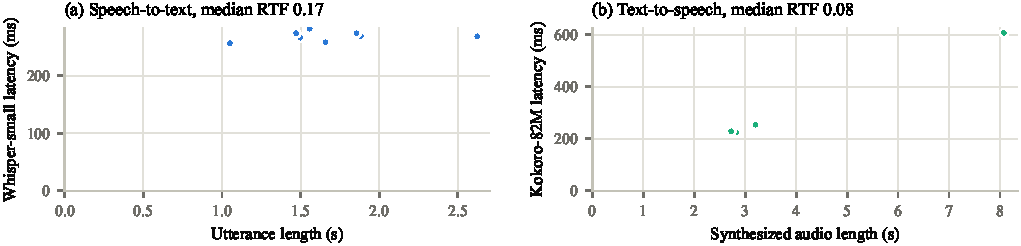
\includegraphics[width=\textwidth]{figures/voice.pdf}
\caption{On-device speech latency. (a) Whisper-small transcribes 1--2.6\,s utterances in about
0.27\,s. (b) Kokoro-82M synthesises speech about 13$\times$ faster than real time.}
\label{fig:voice}
\end{figure*}

Whisper-small transcribed all eight synthetic utterances without word errors in a median 269\,ms
(real-time factor 0.17), and Kokoro-82M synthesised replies in a median 241\,ms (real-time factor
0.079, \cref{fig:voice}). A spoken request therefore flows through recognition
($\approx$0.27\,s), decision ($\approx$0.27--0.30\,s) and the start of synthesis ($\approx$0.25\,s for a
short reply), well under a second, with every stage on device.

% ================================================================ 9 Discussion
\section{Discussion}\label{sec:discussion}

\paragraph{Why narrow works.}
Narrowness turns the hardest parts of an LLM assistant into engineering problems with clean
answers. A fixed prompt makes prefix caching exact and nearly free; a closed intent set with typed
parameters makes constrained decoding small and sound; and typed decisions make authorisation a deterministic
policy rather than a property of model text. The resulting assistant is fast because it reads the
long part of its prompt once, and safe because the model has no path to execution that the policy
does not see.

\paragraph{Caching makes few-shot prompting affordable.}
The ablation and the cost model connect: few-shot examples provide the accuracy, and the prefix
cache removes their latency cost. Without the cache, each example token costs about 1.4\,ms on
every request; with it, examples are paid for once at start-up (or never, with a warm disk cache).
This suggests a general design rule for on-device assistants: put as much of the specification as
possible into a stable prefix, and keep the variable part short.

\paragraph{Limits of the design.}
\begin{itemize}
\item \textbf{Small evaluation sets.} With 40 and 24 cases, one case moves accuracy by 2.5--4.2
  points, and the intervals in \cref{tab:accuracy} overlap.
\item \textbf{Single machine, synthetic speech.} Timings come from one M4. The speech test uses
  synthesised rather than recorded, accented or noisy speech.
\item \textbf{Free-form answers.} \texttt{answer\_question} replies from a 1.7B model are short and
  sometimes imprecise. They are labelled as answers and never executed.
\item \textbf{History reuse needs a stable prefix.} Conversation-level reuse is implemented
  (\cref{sec:convreuse}), but with a sliding history window it only helps the first turns, and the
  block window that keeps it effective cost some accuracy. Neither is on by default.
\item \textbf{Grammars choose values.} A schema grammar always produces \emph{some} legal string,
  so constraining allow-listed values (app names) turns an unknown request into a wrong one. R2
  leaves such values free and lets the gate refuse them.
\item \textbf{Synthetic training data.} The adapter is trained on templated utterances; its
  test-set gain is measured on 60 requests from the same authors (\cref{sec:lora}).
\item \textbf{Same-user trust boundary.} The API token stops browsers and other accounts, not
  processes running as the user (\cref{sec:api}).
\item \textbf{Multi-step planning.} The planner comparison uses 61 dev and 30 fresh requests, so
  its intervals are wide, and the clause planner inherits every single-intent routing error.
\end{itemize}

\paragraph{Threats to validity.}
The dev set influenced prompt design, so its accuracy is optimistic; the fresh set mitigates but
does not remove this, since the final revision was guided by general failure categories observed
on the dev set. Benchmarks ran on a machine with other applications open; we report medians and
show per-request spread, and a run-time watchdog aborted runs if free memory dropped below 25\%.
All measurements in this revision were repeated with the final code (content-derived fingerprint,
schema grammar, strict validation); the cached TTFT (72\,ms) and the 20/20 identical greedy outputs
across cold build, disk load and no cache are unchanged from revision 1. The constraint-mode comparison (\cref{tab:ablation3}) uses the same single model,
machine and evaluation sets as the rest of the paper.

\paragraph{Ethics and privacy.}
All audio, text and preferences stay on the device; no account or network service is required after
the one-time model download. Preferences are stored only after explicit confirmation, and the
assistant cannot read common secret files. The run history of multi-step requests keeps only
metadata and never file contents, diffs or answers.

% ================================================================ 10 Future work
\section{Future Work}

\begin{enumerate}
\item \textbf{History policy:} a multi-turn set with real follow-ups (``open it'', ``why did that
  fail?'') to decide how much history routing needs, and whether a block window with conversation
  reuse~\cite{zheng2024sglang} is worth its accuracy cost. A further step would be to prefill the
  next turn's rendered reply while the answer is spoken.
\item \textbf{KV quantisation at long context:} 8-bit KV is free on accuracy but gives no
  speed-up below 8k tokens (\cref{sec:kvvariants}); per-channel key quantisation~\cite{liu2024kivi,hooper2024kvquant}
  may rescue 4-bit, and longer sessions may make it pay off.
\item \textbf{Multi-step evaluation:} a multi-step set written by someone other than the
  authors, and recorded spoken multi-step requests.
\item \textbf{Clarification:} a contrastive set of vague vs.\ destructive requests, and
  hand-written (not templated) training data for the adapter of \cref{sec:lora}.
\item \textbf{Wake word:} a ``Hey R2'' detector on top of push-to-talk.
\item \textbf{Decode speed:} speculative decoding~\cite{leviathan2023speculative} for longer spoken
  answers.
\item \textbf{Larger studies:} more requests, recorded speech, several Apple chips and other small
  models.
\end{enumerate}

% ================================================================ 11 Conclusion
\section{Conclusion}

R2 shows that a small local model can feel like a native voice assistant when the system around it
is designed for a narrow task. A persistent prefix KV cache turns a 1.5\,s prompt into a 72\,ms
response start with identical outputs. Its behaviour follows from a few lines of theory: prefix
invariance, the KV memory formula and a linear-plus-quadratic cost model. Few-shot examples deliver
91.7\% exact accuracy on a fresh set and 85.0\% on a harder test set, a schema grammar keeps that accuracy under strict
validation, and a fail-closed policy keeps every action, including each step of a multi-step
request, under the user's control.

% ================================================================ back matter
\section*{Reproducibility}\label{sec:repro}
All numbers in this paper are produced by scripts in the repository and stored in
\texttt{artifacts/}:
\begin{lstlisting}[language=bash,numbers=none,basicstyle=\ttfamily\scriptsize]
uv sync && uv run python -m pytest          # 252 tests
uv run python training/bench_kv.py           # Table 3, Fig. 3
uv run python training/bench_scaling.py      # Table 4, Figs. 4-5
uv run python training/bench_conversation.py # conversation reuse table
uv run python training/bench_kv_variants.py  # kv_bits, rotating windows
uv run python training/evaluate.py --backend mlx [--eval data/eval_{fresh,test}.jsonl]
uv run python training/ablation.py           # few-shot x constraint, 3 sets
uv run python training/synth_data.py         # synthetic LoRA data
uv run python training/train.py --yes        # LoRA, cached model only
uv run python training/compare_lora.py       # base vs adapter, McNemar
uv run python training/eval_multistep.py --backend mlx [--data data/eval_multistep_fresh.jsonl]
uv run python training/bench_voice.py        # Fig. 11
uv run python paper/make_figures.py          # all figures
\end{lstlisting}

\section*{Author Contributions}
\textbf{Siavash Shokrtalab} (full-stack engineering): system architecture, Python core and
HTTP API, SwiftUI macOS client, voice pipeline integration, tooling and testing.
\textbf{Alireza Panahdoost} (research and machine learning): research questions, KV cache and
constrained-decoding methodology, theoretical analysis, benchmark and evaluation design, error
analysis. Both authors wrote and approved the manuscript.

\section*{Revision History}
\textbf{Revision 2} follows an external review of the code and of revision 1. It adds token, Host
and Origin checks to the local API and binds confirmations to a single-use, expiring id
(\cref{sec:safety}); derives the cache fingerprint from content and validates every cache layer,
with atomic writes and on-disk eviction (\cref{sec:impl}); rejects unknown parameters and adds
schema-constrained decoding with its ablation (\cref{sec:constrained,sec:ablation}); hardens the
file tools against links and races; adds bounded multi-step requests with a client view (\cref{sec:agent}); measures
conversation-level KV reuse (\cref{sec:convreuse}), quantised KV and rotating windows
(\cref{sec:kvvariants}); adds a 60-request test set and a LoRA comparison with its rationale and parameter
count (\cref{sec:lora}); and states why existing assistants do not meet R2's requirements
(\cref{sec:why}).
All measurements were repeated with the final code.

\section*{Acknowledgements}
We thank the developers of MLX, mlx-lm, Qwen3, Whisper and Kokoro for releasing their work openly.
Parts of the implementation and of this manuscript were prepared with the help of an AI coding
assistant; the authors are responsible for all content.

{\small
\bibliographystyle{unsrtnat}
\bibliography{references}
}

\clearpage
\onecolumn
\appendix
\section{System Prompt Excerpt}\label{app:prompt}

\begin{lstlisting}[language={},numbers=none,basicstyle=\ttfamily\scriptsize,breaklines=true]
You are R2, a narrow, local macOS developer assistant (like Siri, but only for developer tasks in the
user's active workspace).

Turn the user's request into exactly ONE JSON object and nothing else:
{"intent": "<intent>", "parameters": {...}}

Intents (parameters) - when to use:
- general_help {} - ONLY when the user asks about R2 itself: what you can do / how to use you
- git_status {} - branch, repo status, uncommitted or changed files
- git_diff_summary {} - summary or size of the diff / what changed in the code
- search_files {"pattern": "<glob, e.g. *.py, *test*, README*>"} - find, list or locate files by name or type
- read_file {"path": "<relative file path>"} - show, read, print or display the contents of a specific file
- open_app {"app_name": "<one of the approved apps>"} - launch or open an application
- remember_preference {"key": "<snake_case key>", "value": "<value>"} - user tells you a personal preference ...
- recall_preference {"key": "<snake_case key>"} - user asks about their OWN previously saved preference ...
- answer_question {"question": "<the user's question>"} - a software-development knowledge question ...
- clarify_request {"question": "<short follow-up question>"} - a vague command whose target is unclear ...
- unsupported {"reason": "<short reason>"} - chit-chat, trivia, math, destructive or out-of-scope requests
... approved apps, rules, and 25 worked examples (675 tokens) follow.
\end{lstlisting}

\section{Local HTTP API}

Every route except \texttt{/health} requires \texttt{Authorization: Bearer <token>}; see
\cref{sec:api} for the Host, Origin and content-type rules.

\begin{center}\small
\begin{tabular}{@{}lll@{}}
\toprule
Method & Path & Purpose \\
\midrule
GET & \texttt{/health}, \texttt{/status}, \texttt{/voices} & liveness (no token); model and KV cache state; voice list \\
POST & \texttt{/ask} \{\texttt{text}, \texttt{confirmation\_id}?, \texttt{allow\_runs}?\} & text request $\to$ reply, speech, intent, metrics, confirmation id; may start a run \\
POST & \texttt{/confirm} \{\texttt{confirmation\_id}\}, \texttt{/cancel}, \texttt{/reset} & approve the pending action by id; cancel; clear history \\
POST & \texttt{/ask\_audio} (WAV, $\le$16\,MB) & Whisper transcription, then \texttt{/ask} \\
POST & \texttt{/tts} \{\texttt{text}, \texttt{voice}, \texttt{speed}\} & Kokoro speech as WAV (speed 0.5--2.0) \\
POST & \texttt{/run} \{\texttt{text}\} & plan and start a multi-step run \\
GET & \texttt{/runs/<id>} & poll a run (never returns the confirmation id) \\
POST & \texttt{/runs/<id>/confirm}, \texttt{/cancel} & approve the paused step by id; cancel the run \\
\bottomrule
\end{tabular}
\end{center}

\section{Evaluation Set Composition}

\begin{center}\small
\begin{tabular}{@{}lrrrr@{}}
\toprule
Intent & Dev & Fresh & Test & Synthetic train \\
\midrule
\texttt{git\_status} & 4 & 2 & 6 & 53 \\
\texttt{git\_diff\_summary} & 3 & 2 & 5 & 41 \\
\texttt{search\_files} & 5 & 2 & 8 & 85 \\
\texttt{read\_file} & 4 & 2 & 7 & 91 \\
\texttt{open\_app} & 3 & 2 & 5 & 76 \\
\texttt{remember\_preference} & 3 & 2 & 5 & 61 \\
\texttt{recall\_preference} & 2 & 2 & 4 & 40 \\
\texttt{answer\_question} & 0 & 3 & 5 & 65 \\
\texttt{general\_help} & 3 & 1 & 3 & 38 \\
\texttt{clarify\_request} & 3 & 2 & 4 & 34 \\
\texttt{unsupported} & 10 & 4 & 8 & 116 \\
\midrule
\textbf{Total} & \textbf{40} & \textbf{24} & \textbf{60} & \textbf{700} \\
\bottomrule
\end{tabular}
\end{center}

\end{document}
